\documentclass[11pt, english]{beamer}
\usepackage{babel}
\usepackage[T1]{fontenc}
\usepackage[utf8]{inputenc}

%Justificación del texto
\usepackage{ragged2e}
\justifying

\usepackage{pgf,pgfpages}
\usepackage{pgffor} % For loops
\usepackage{tikz}
\usetikzlibrary{arrows,shapes,backgrounds,calc}

\usepackage{graphicx}
\usepackage{colortbl}
\usepackage{units}

% Fuente caligráfica en entornos matemáticos
\usepackage[cal=boondox,scaled=1.15]{mathalfa}

%% Beamer style >>>>>>>>>>>>>>>>>>>>>>>>>
\mode<presentation>
{
  \usetheme{PHD}
  \setbeamercovered{transparent}
  \setbeamertemplate{items}[square]
}

%\usefonttheme[onlymath]{serif}

\beamertemplatenavigationsymbolsempty

\defbeamertemplate{enumerate item}{mycircle}
{
  %\usebeamerfont*{item projected}%
  \usebeamercolor[bg]{item projected}%
  \begin{pgfpicture}{0ex}{0ex}{1.5ex}{0ex}
    \pgfcircle[fill]{\pgfpoint{-0.1pt}{.65ex}}{1.1ex}
    \pgfbox[center,base]{\color{PHDyellowd}{\insertenumlabel}}
  \end{pgfpicture}%
}
[action]
{\setbeamerfont{item projected}{size=\scriptsize}}
\setbeamertemplate{enumerate item}[mycircle]

\title{Neural Networks}
\author{Álex Pérez Fernández, Rafa Rodríguez Galván}


% PDFLaTeX font choosing
\usepackage[default, scale=1.0]{lato}

% \usepackage{array, multirow, rotating} % booktabs: toprule, midrule...
\usepackage{array,booktabs,tabularx}

\usepackage{current-definitions}
\usepackage{neural-networks}

\newtheorem{remark}{Remark}
\newtheorem{proposition}{Proposition}
%\newtheorem{theorem}{Theorem}

% Presentation goodies >>>>>>>>>>>>>>>>>>>>>>>>>>>>
\newcommand<>{\myframed}[1]{\alt#2{\tikz[phd] \node[box] {#1};}{{#1}}}
\newcommand<>{\myframedAlert}[1]{\alt#2{\tikz[phdB] \node[boxB] {\color{black}#1};}{{#1}}}
\newcommand<>{\framedmath}[1]{%
\alt#2{\tikz[phd] \node[box] {\ensuremath{#1}};}{\ensuremath{#1}}}
\newcommand{\framedB}[1]{\tikz[phd] \node[boxB] {#1};}
\newcommand{\framedmathB}[1]{\framedB{\ensuremath{\displaystyle{#1}}}}
\newcommand{\ver}[1]{\footnote{See #1}}
\newcommand{\cita}[1]{{\color{PHDgray}\cite{#1}}}
\newcommand\cellalert[2]{\only<#1>{\cellcolor{PHDyellow}}\alt<#1>{\textbf{#2}}{#2}}
\newcommand{\soften}[1]{{\color{PHDgray}#1}}
\newcommand{\rowalert}[7]{%
    \cellalert{#1}{#2} & \cellalert{#1}{#3} &
    \cellalert{#1}{#4} & \cellalert{#1}{#5} &
    \cellalert{#1}{#6} & \cellalert{#1}{#7}}

% \usepackage{wasysym}
% \newcommand{\good}{{\color{PHDgreen}$\CIRCLE$}} %\blacksmiley
% \newcommand{\bad}{{\color{PHDred}$\CIRCLE$}}
\usepackage{pifont, fontawesome}
\newcommand{\good}{{\color{PHDgreen}\ding{52}}}
\newcommand{\bad}{{\color{PHDred}\ding{56}}}
\newcommand{\exclamation}{{\large\color{PHDred}{\textbf{\itshape !}}}}
\newcommand{\question}{{\large\color{PHDred}{\textbf{\itshape ?}}}}
\newcommand\colorUnderLine[2][PHDyellow]{\color{#1}\underline{{\color{black}#2}}\color{black}\xspace}
\newcommand\gris[1]{{\color{PHDgray}#1}}
\newcommand\amarillo[1]{{\color{PHDyellow}#1}}
\newcommand\tiragris[1]{{\par\hfill\small\gris{#1}}}
\newcommand\point{\alert{\faHandORight}\xspace}
%<<<<<<<<<<<<<<<

\setcounter{tocdepth}{1}


%
% Bibliography
%
%\usepackage{natbib}

% To list each bibliographic entry in a line
\setbeamertemplate{bibliography entry title}{}
\setbeamertemplate{bibliography entry location}{}
\setbeamertemplate{bibliography entry note}{}

% ... end of preamble.

\AtBeginSection{\frame{\sectionpage}}

\colorlet{inputcolor}{green!60!black}
\colorlet{hiddencolor}{blue!60!black}
\colorlet{outcolor}{red!60!black}

%--------------------------------------------------------------
\begin{document}
%--------------------------------------------------------------

% Tikz style and beamer template ------->>>
\tikzstyle{every picture}+=[remember picture]
\tikzstyle{na} = [baseline=-.5ex]
\tikzstyle{phd} = [baseline=-.6ex,
  box/.style={rectangle, draw=PHDblueC, thick, fill=PHDblueA,
    align=center, rounded corners, minimum height=1.6em},
  boxB/.style={rectangle, draw=PHDredA, thick, fill=PHDblueA,
    align=center, rounded corners, minimum height=1.6em}]
\tikzstyle{phdB} = [baseline=-.7ex,
  box/.style={rectangle, draw=PHDblueC, thick, fill=PHDblueA,
    align=center, rounded corners, minimum height=1.6em},
  boxB/.style={rectangle, draw=PHDredA, thick, fill=PHDblueA,
    align=center, rounded corners, minimum height=1.6em}]
\tikzstyle{myarrow} = [->,>=latex, PHDredA, shorten >=4pt,
  opacity=.6, line width=0.6mm]
\tikzstyle{myarrow2} = [->,>=latex, PHDblueC, shorten >=4pt, opacity=.2, line width=0.4mm]
\tikzstyle{myarrow3} = [
     opacity=.7,
%    >=triangle 60,              % Nice arrows; your taste may be different
    node distance=6mm and 60mm, % Global setup of box spacing
    every join/.style={norm},   % Default linetype for connecting
                                % boxes
    line width=0.6mm,
    PHDredA,
    ->
    ]
\setbeamertemplate{background}
 {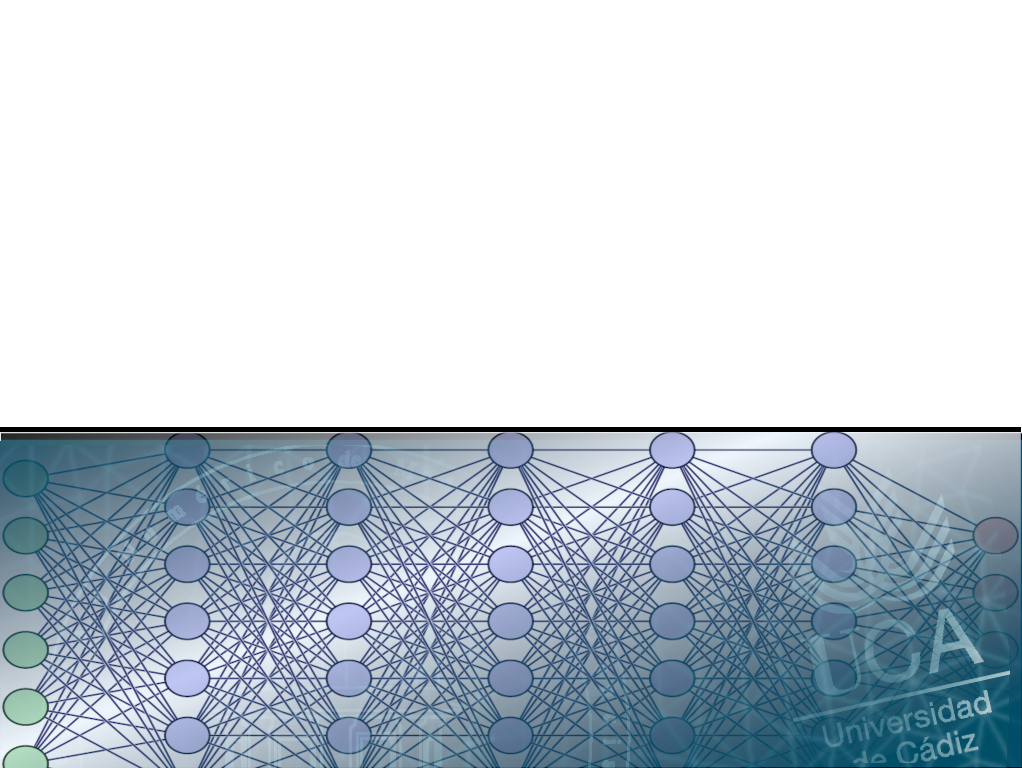
\includegraphics[width=\paperwidth,height=\paperheight]{frontpage_bg}}
\setbeamertemplate{footline}[default]
% <<<-------


% Write custom titlepage ------->>>
\begin{frame}
  \titlepage
  \vspace{5cm}
\end{frame}

% Set the background for the rest of the slides.
\setbeamertemplate{background}{}
 % {
\includegraphics[width=\paperwidth,height=\paperheight]{slide_bg}}


% Write all of the slides..........

% \begin{frame}{Outline}
%   \tableofcontents
% \end{frame}

% Start inserting infoline at the end
\setbeamertemplate{footline}[PHDtheme]
% <<<-------

\newcommand{\imgdir}{Undefined, use renewcommand!}

%--------------------------------------------------------------
\section{Neural Networks}
%--------------------------------------------------------------

\begin{frame}{Neural Networks...}
%--------------------------------------------------------------
  \vspace{-0.9em}
  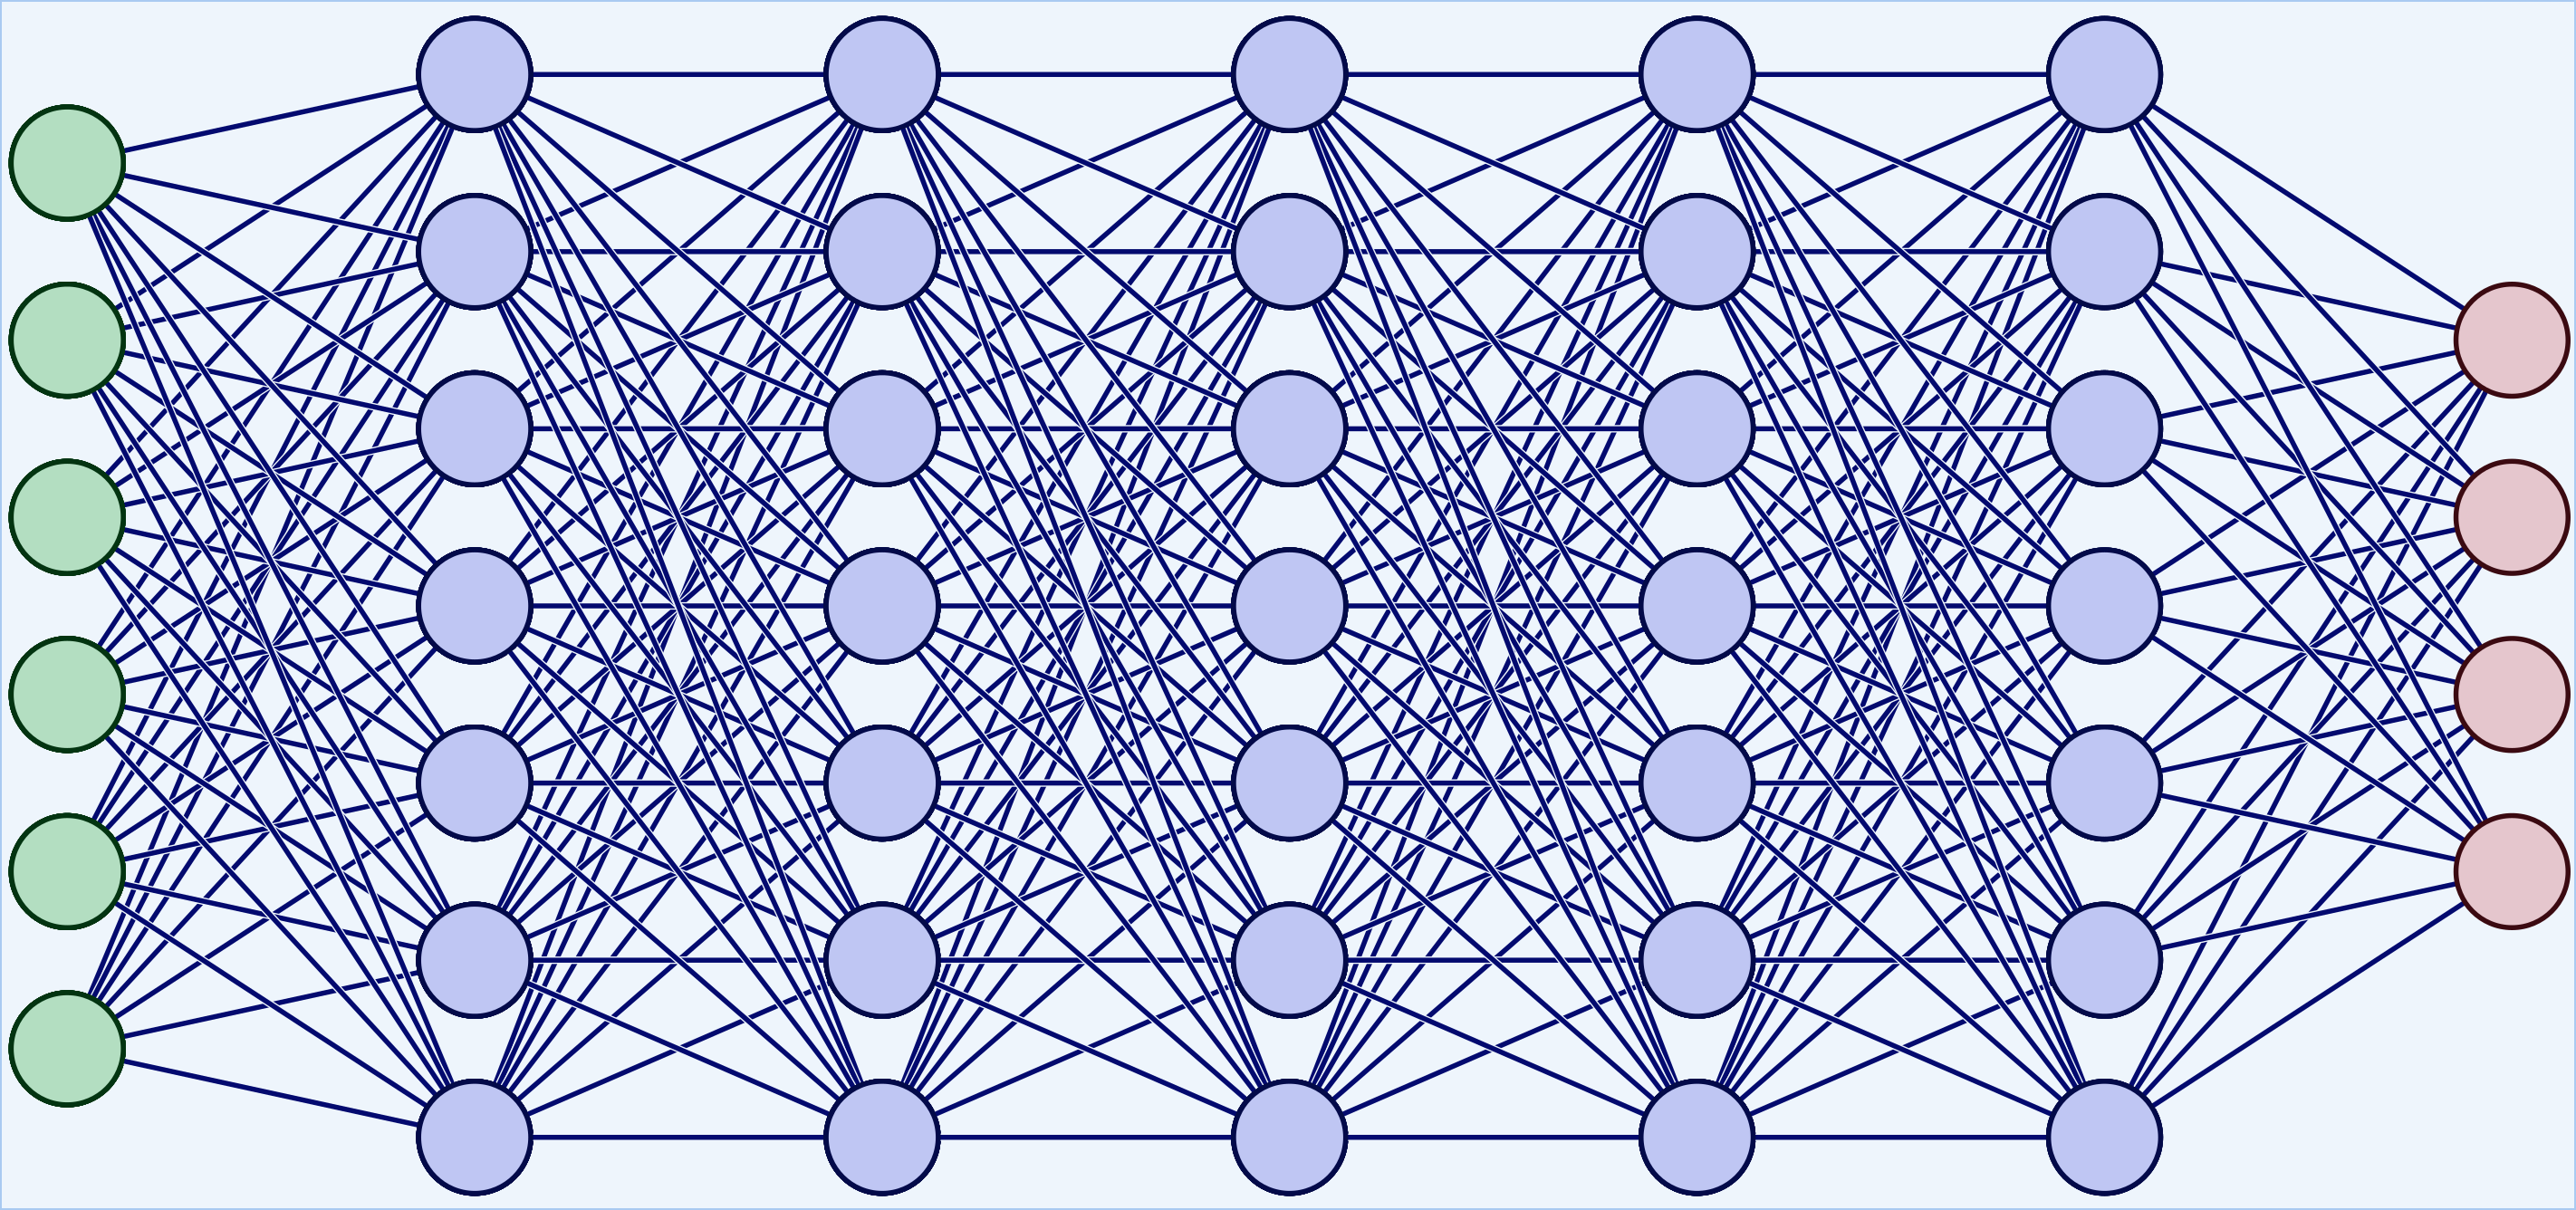
\includegraphics[width=0.95\linewidth]{deep-NN}
  \pause
  ~
  \vfill
  {\large\textbf{...are mathematical artifacts:}}
  \begin{gather*}
    {\color{inputcolor} \xx} \mapsto 
    {\color{hiddencolor}\ff_1({\color{inputcolor} \xx})} \mapsto 
    {\color{hiddencolor}\ff_2\circ \ff_1({\color{inputcolor} \xx})} \mapsto 
    % {\color{hiddencolor}\ff_3\circ \ff_2\circ \ff_1({\color{inputcolor} x})} \mapsto \pause
    {\color{hiddencolor} \cdots} \mapsto
    {\color{hiddencolor} \ff_L\circ \cdots \circ \ff_2\circ \ff_1({\color{inputcolor} x})} = {\color{outcolor}\mathbf{y}}
  \end{gather*}
\end{frame}

\begin{frame}
  \vspace{-0.2em}
  \begin{flushright}
  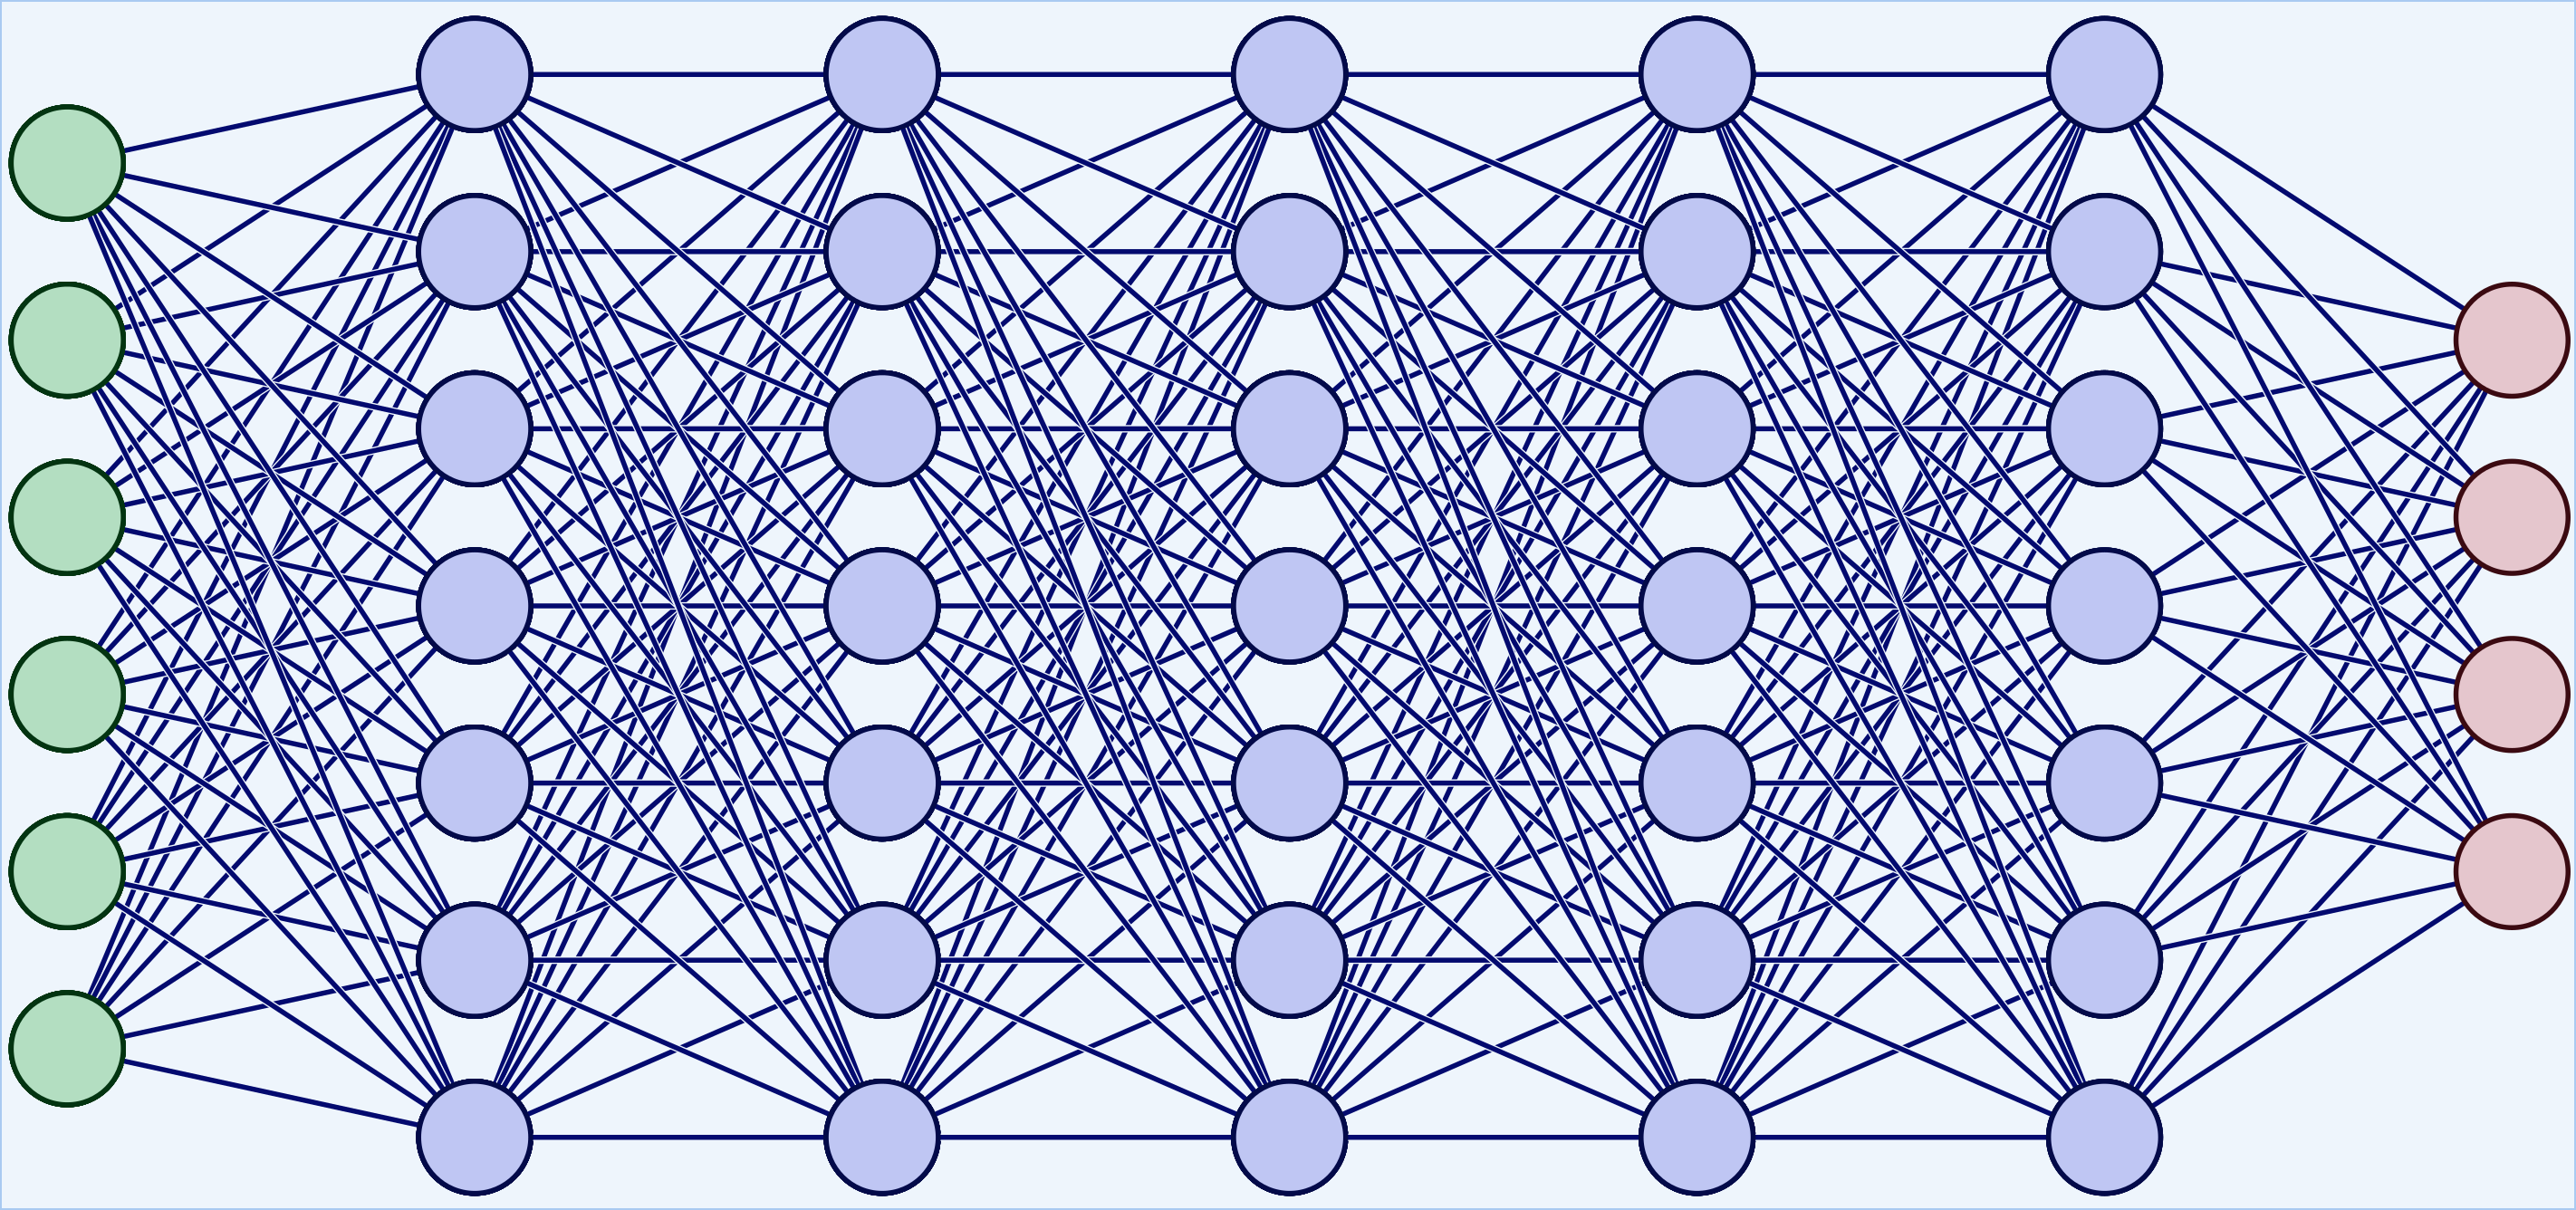
\includegraphics[width=0.52\linewidth]{deep-NN}
  \end{flushright}
  \vspace{-0.7em}
  {\large\textbf{Definición}}:\par
  una \structure{\bf Red Neuronal} (\textit{RN} o \textit{NN}) es una función $f_{NN}:\Rset^n \to \Rset^m$ del tipo:
    $$
    {\color{outcolor}\mathbf{y}} = f_{NN}({\color{inputcolor}x}) = 
    {\color{hiddencolor} \ff_L\circ \cdots \circ \ff_2\circ \ff_1({\color{inputcolor} x})}.
    $$
  Donde...
  \begin{itemize}\itemsep=0.5em
    \item Cada función $\ff_i$ se llama una \textbf{capa} (
      {\color{inputcolor}entrada} $\rightarrow$
      {\color{hiddencolor}oculta} $\rightarrow$ 
      {\color{outcolor}salida} )
    \item Cada capa $\ff_i$ está compuesta por un nº variable de \textbf{neuronas}
    \item Cada neurona depende un conjunto de \textbf{parámetros}, que determinarán a la RN 
  \end{itemize} 
  \bigskip
  \scriptsize
  \begin{flushright}
  $\star$ La RN de la figura  se dice de tipo «\textit{feed forward}» o {prealimentada}
  \end{flushright}
\end{frame}

\begin{frame}{Un ejemplo}
  \vspace{-0.5em}
  \begin{center}
  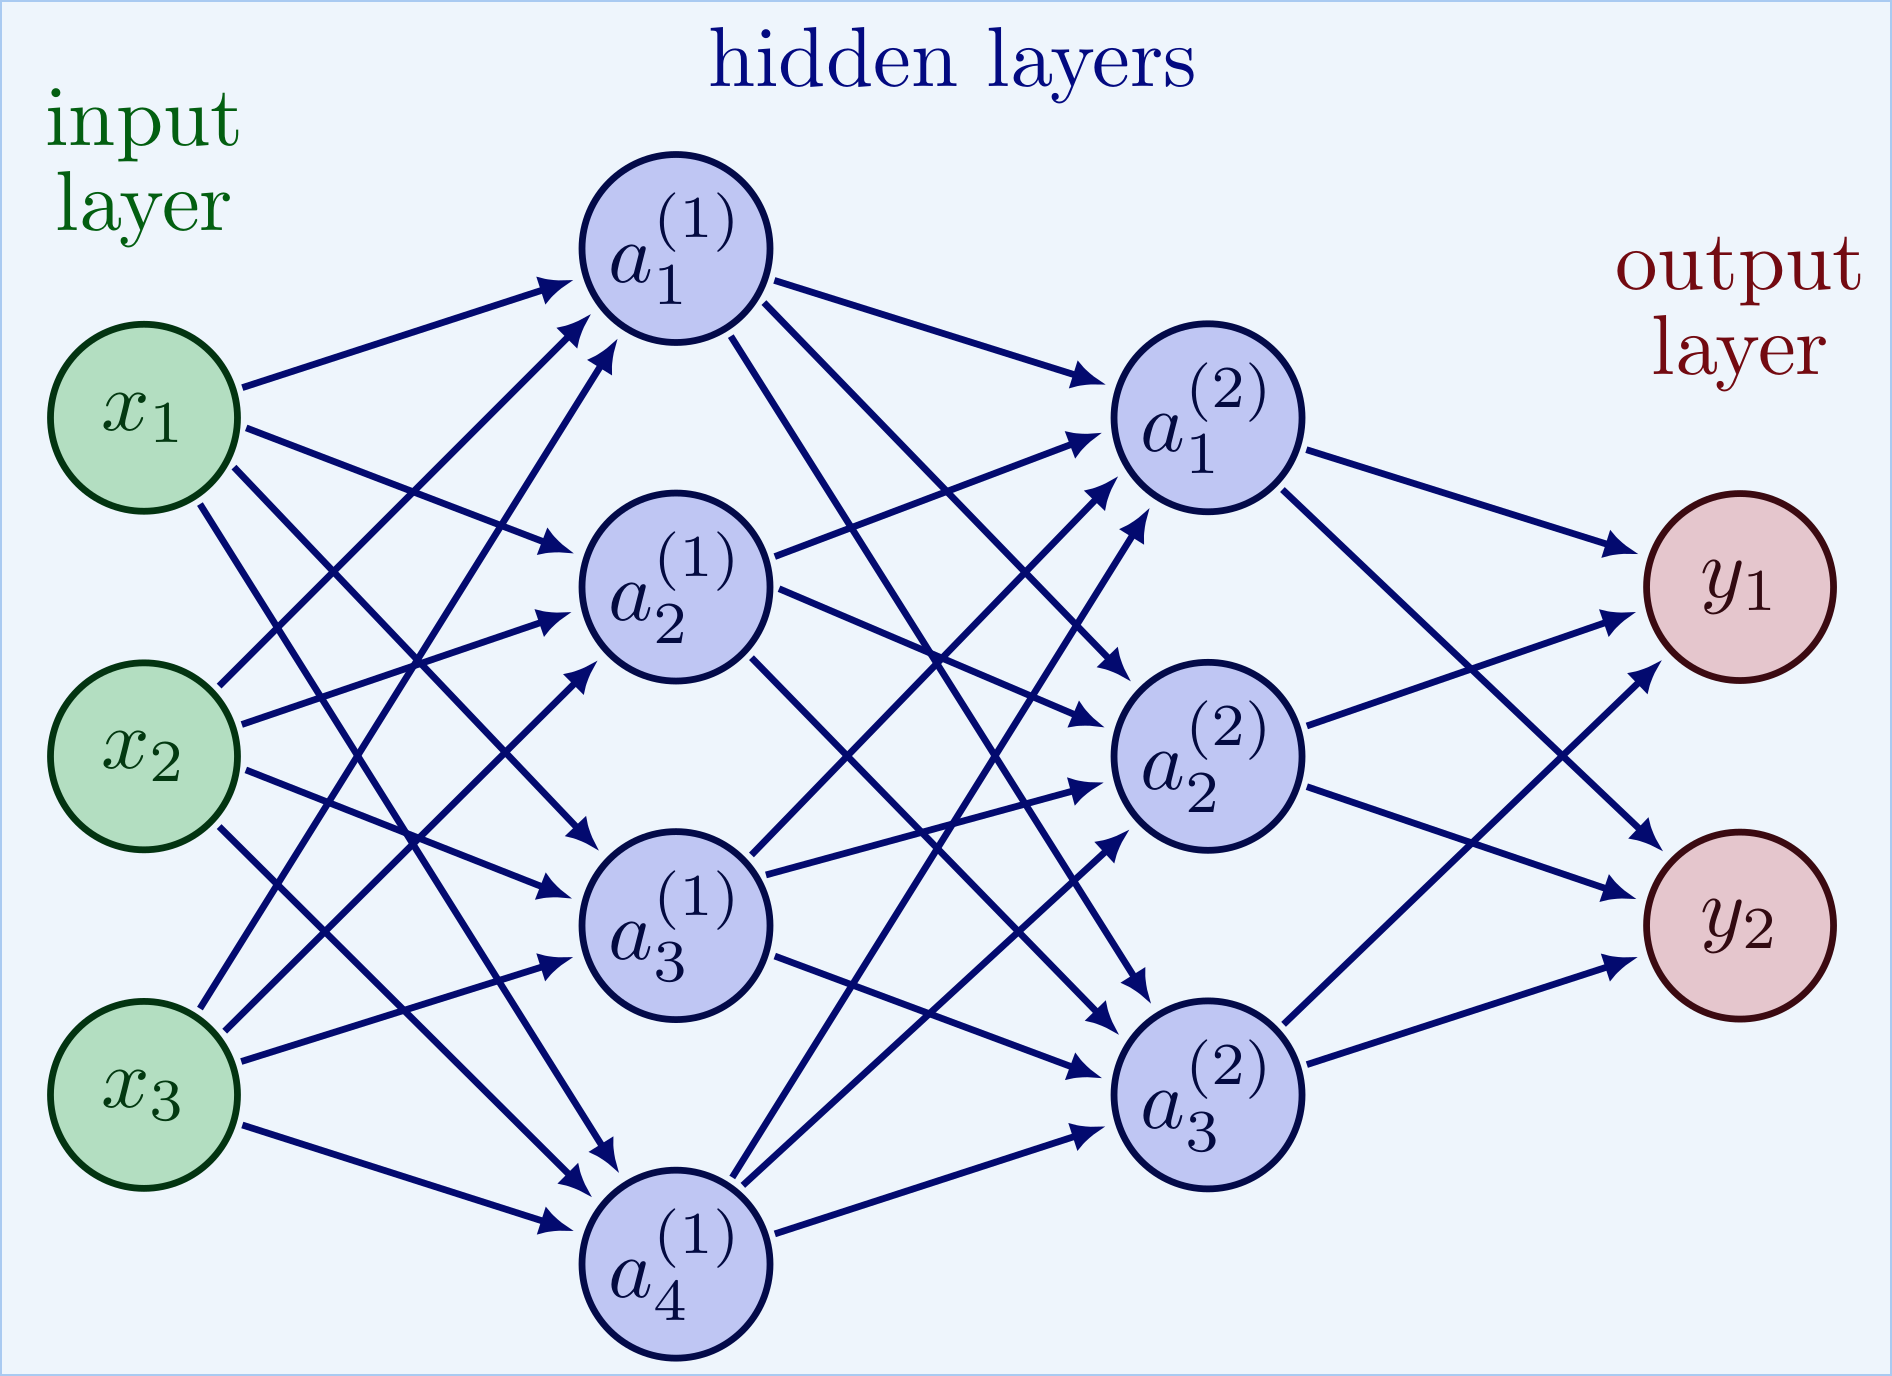
\includegraphics[width=0.82\linewidth]{example-NN}
  \end{center}
  $$
  f_{NN}:\Rset^3 \to \Rset^2
  \mbox{con $2$ capas ocultas de $4$ y $3$ neuronas}
  $$
\end{frame}


\begin{frame}{Neurona o \emph{perceptrón} simple}
  Cada neurona $j$ de una capa oculta $f_i$ (o de salida $y_i$) es una función% 
  \footnote{Donde $N_i$ es el número de neuronas de la capa $i-1$}:
  $$
  \xx\in \Rset^{N_{i}} \rightarrow \alert{a_j^{(i)}}(\xx) \in \Rset,
  $$
  composición de%
  \begin{itemize}
    \item una función afín con parámetros $\structure{\ww}=({w_1},\dots,{w_{N_i}})$ y \structure{$b$}
    \item una función no lineal $\sigma$, llamada «\structure{función de activación}»  
  \end{itemize}
  \begin{block}{}
    \vspace{-0.8em}
  \begin{align*}
    \alert{a_j^{(i)}}(\xx) &= \sigma(w_1 x_1 + w_2 x_2 + \cdots + w_{N_i} x_{N_i} + b) = \\
                   &=\sigma\Big(\sum_{k=1}^{N_i} w_k x_k +b\Big) = \sigma(\ww\cdot\xx + b)
  \end{align*}
  \end{block}
\end{frame}

\begin{frame}{Con más propiedad...}
Para aligerar la notación se omitieron los índices correspondientes a la capa, $i$, y a la neurona, $j$. Debería ser:
  \begin{align*}
    \alert{a_j^{(i)}}(\xx) = \sigma\Big(\sum_{k=1}^{N_i} w^{(i)}_{j,k} x_k +b^{(i)}_j\Big).
    % = \sigma\big(\ww^{(i)}\cdot\xx + b^{(i)}_j\big)
  \end{align*}
  Así, si $\WW^{(i)}$ denota a la matriz de valores $w^{(i)}_{j,k}$, y $\vect b^{(i)}$ es el vector $(b^{(i)}_j)$, podemos escribir a tod la \alert{capa} $i$ como:
$$
\alert{\ff_i(\xx)} = {\boldsymbol\sigma_i}(\WW^{(i)}\xx + \vect b^{(i)})
$$
La RN está determinada por los parámetros $\WW^{(i)}$, los desplazamientos $\vect b^{(i)}$ y las funciones de activación $\boldsymbol\sigma_i$
\end{frame}

\section{Partes básicas de una red neuronal}

%\alert{descenso de gradiente}\footnote{\url{https://en.wikipedia.org/wiki/Gradient_descent}}
\begin{frame}{Funciones de activación}
Es una abstración que representa la \structure{\bf tasa potencial de acción.}
\begin{center}
  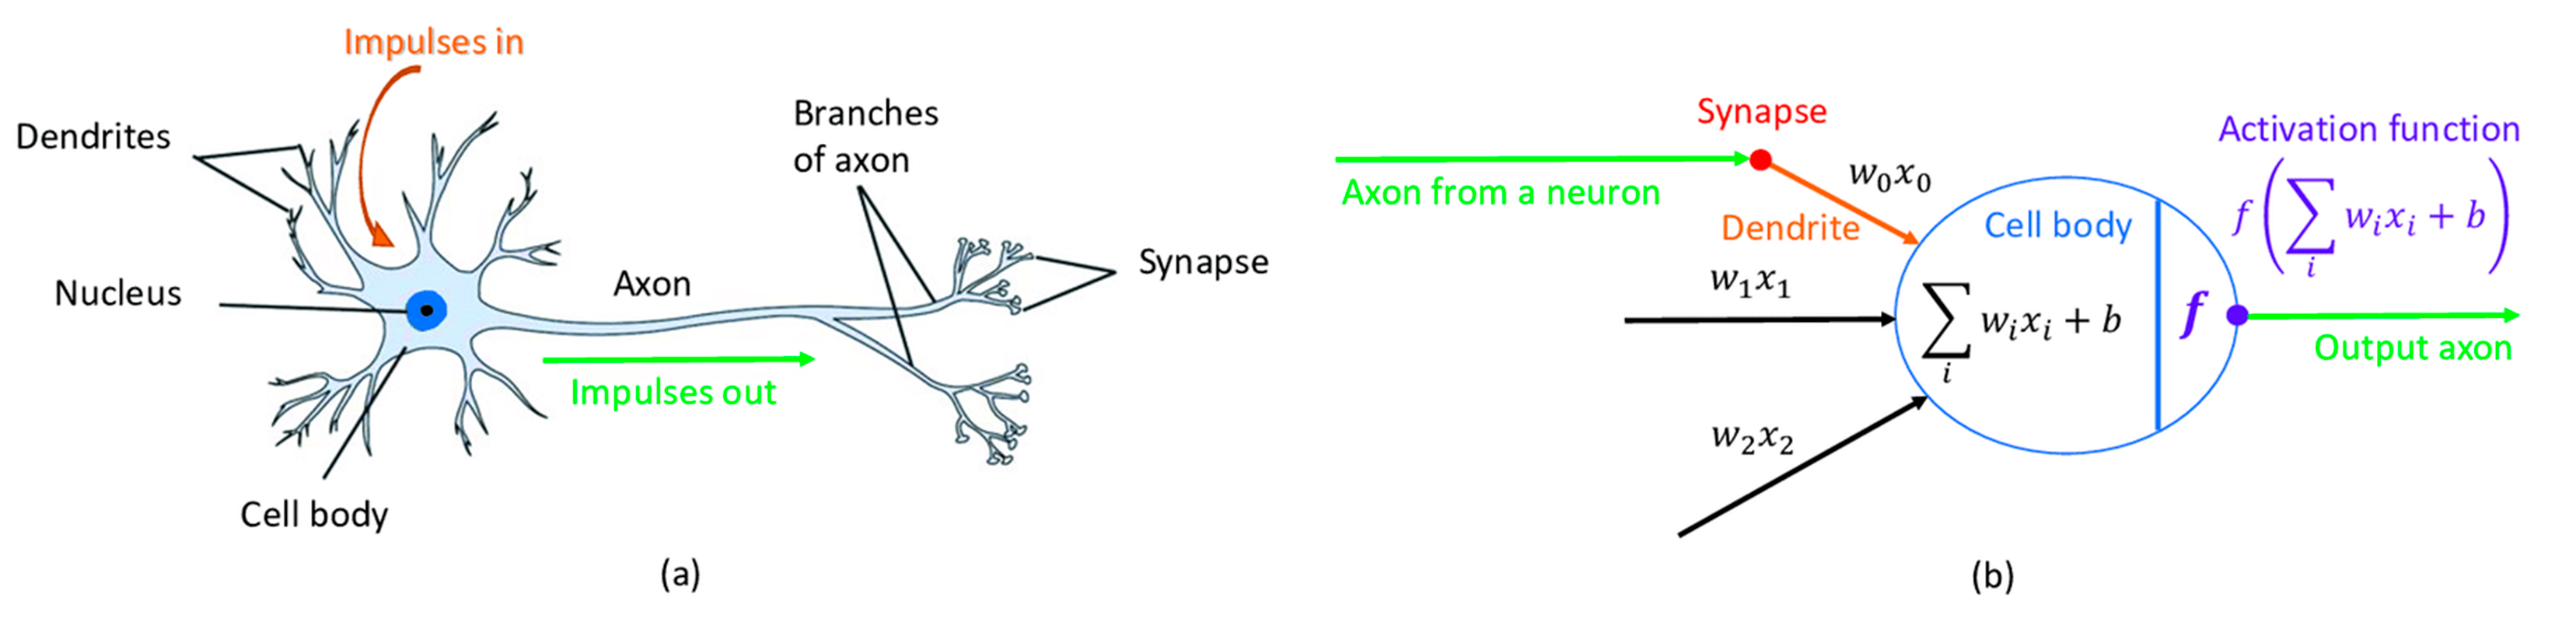
\includegraphics[width=1\linewidth]{src/Activation-IMG-1.png}
  \footnote{\href{https://www.researchgate.net/publication/317679065_Ranking_to_Learn_and_Learning_to_Rank_On_the_Role_of_Ranking_in_Pattern_Recognition_Applications}{Ranking to Learn and Learning to Rank: On the Role of Ranking in Pattern Recognition Applications}}
\end{center}
Dada una entrada se procesa \textbf{(parte lineal)} y se valora si la neurona dispara o no \alert{perceptron}. Para comportamientos más complejos podemos devolver una probabilidad
si es baja menos probable es que dispare y viceversa, de ahí proviene la \alert{función de activación sigmoidal.}
\end{frame}

\begin{frame}{¿Por qué necesitamos funciones de activación?}
  Supongamos que no tenemos funciones de activación, luego la red neural es composición de aplicaciones lineales, esto implica que \structure{\bf la
  red es una función lineal.}
  $$f_{NN}({\color{inputcolor}x}) = {\color{hiddencolor}w_1 x_1 + w_2 x_2 + \cdots + w_{N_i} x_{N_i} + b}$$
  Por lo tanto, no importa cuantas capas tenga el modelo, puesto que estamos realizando una transformación lineal en las entradas.
  Esto es un problema, puesto que no podemos \alert{modelar problemas no lineales}.

  % Ejemplo de problemas no lineales y lineales por ejemplo de ajustar ecuaciones o similar.

\end{frame}

\begin{frame}{Representación de funciones de activación}
  \vspace{-0.7em}
  \begin{center}
  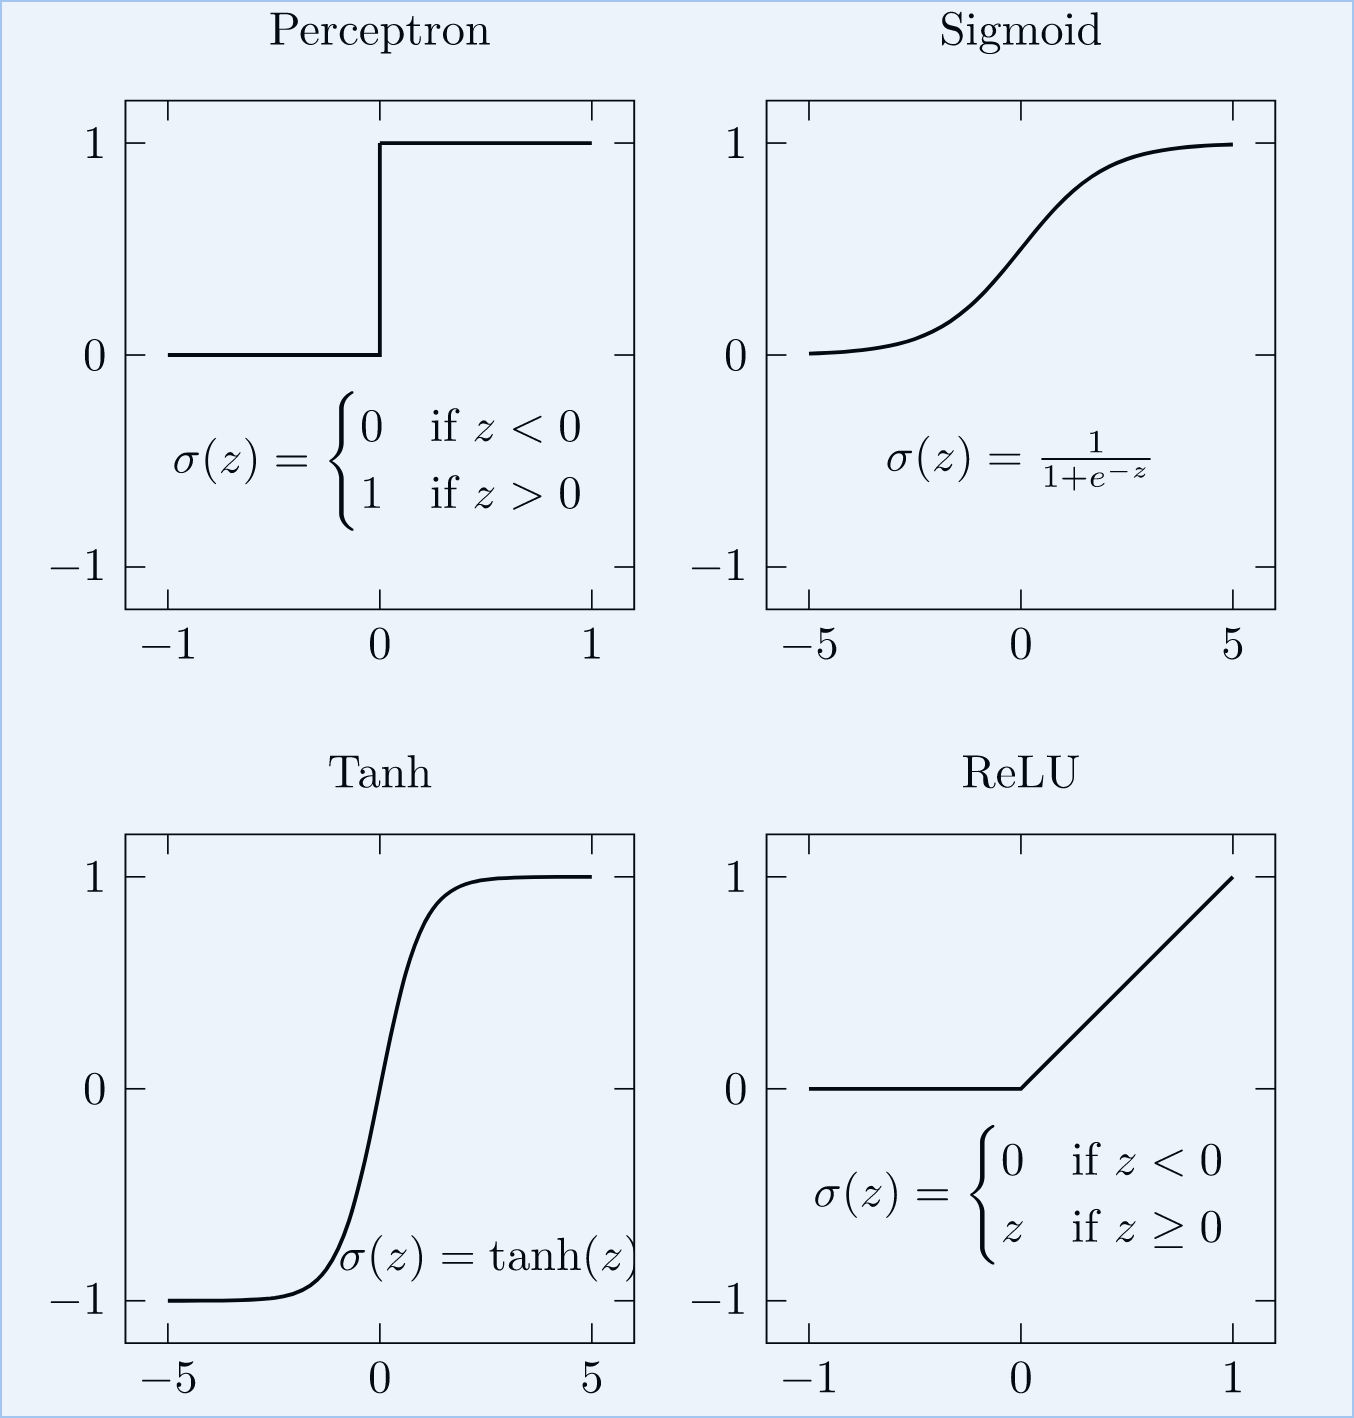
\includegraphics[width=0.65\linewidth]{funciones_activacion}
  \end{center}
\end{frame}

\begin{frame}{Funciones de perdida}
Una función de perdia compara la salida de la red neuronal con la salida esperada, y nos dice que tan \structure{\bf bien o mal lo esta haciendo la red neuronal.}

\vspace*{0.8em}

Cuando entrenamos, nuestro objetivo es \alert{minimazar la perdida entre la salida esperada y la salida de la red neuronal.}

\vspace*{0.8em}

Ejemplos:
\begin{itemize}
  \item Problema de regresión $$
  y_{pred}=\begin{pmatrix}
    250 & 300 \\
    300 & 400 \\ 
  \end{pmatrix}
  \hspace*{0.8em}
  y_{real} = \begin{pmatrix}
    100 & 150 \\
    400 & 200 \\
  \end{pmatrix}
  $$
  \item Problema de clasificación
  $$
  y_{pred}=\begin{bmatrix}
    0.12 \\
    0.48 \\
    0.4 \\ 
  \end{bmatrix}
  \hspace*{0.8em}
  y_{real} = \begin{bmatrix}
    0 \\
    1 \\
    0 \\
  \end{bmatrix}
  $$
\end{itemize}
\end{frame}

\begin{frame}
  Podemos pensarlo como un residuo en estadística, que se encarga de  medir la distancia entre los \textbf{valores actuales de y y los de la linea de regresión} (valores predecidos).
  
  \vspace{0.8em}

  \textbf{El objetivo es minimizar la distancia neta.}
  \begin{center}
    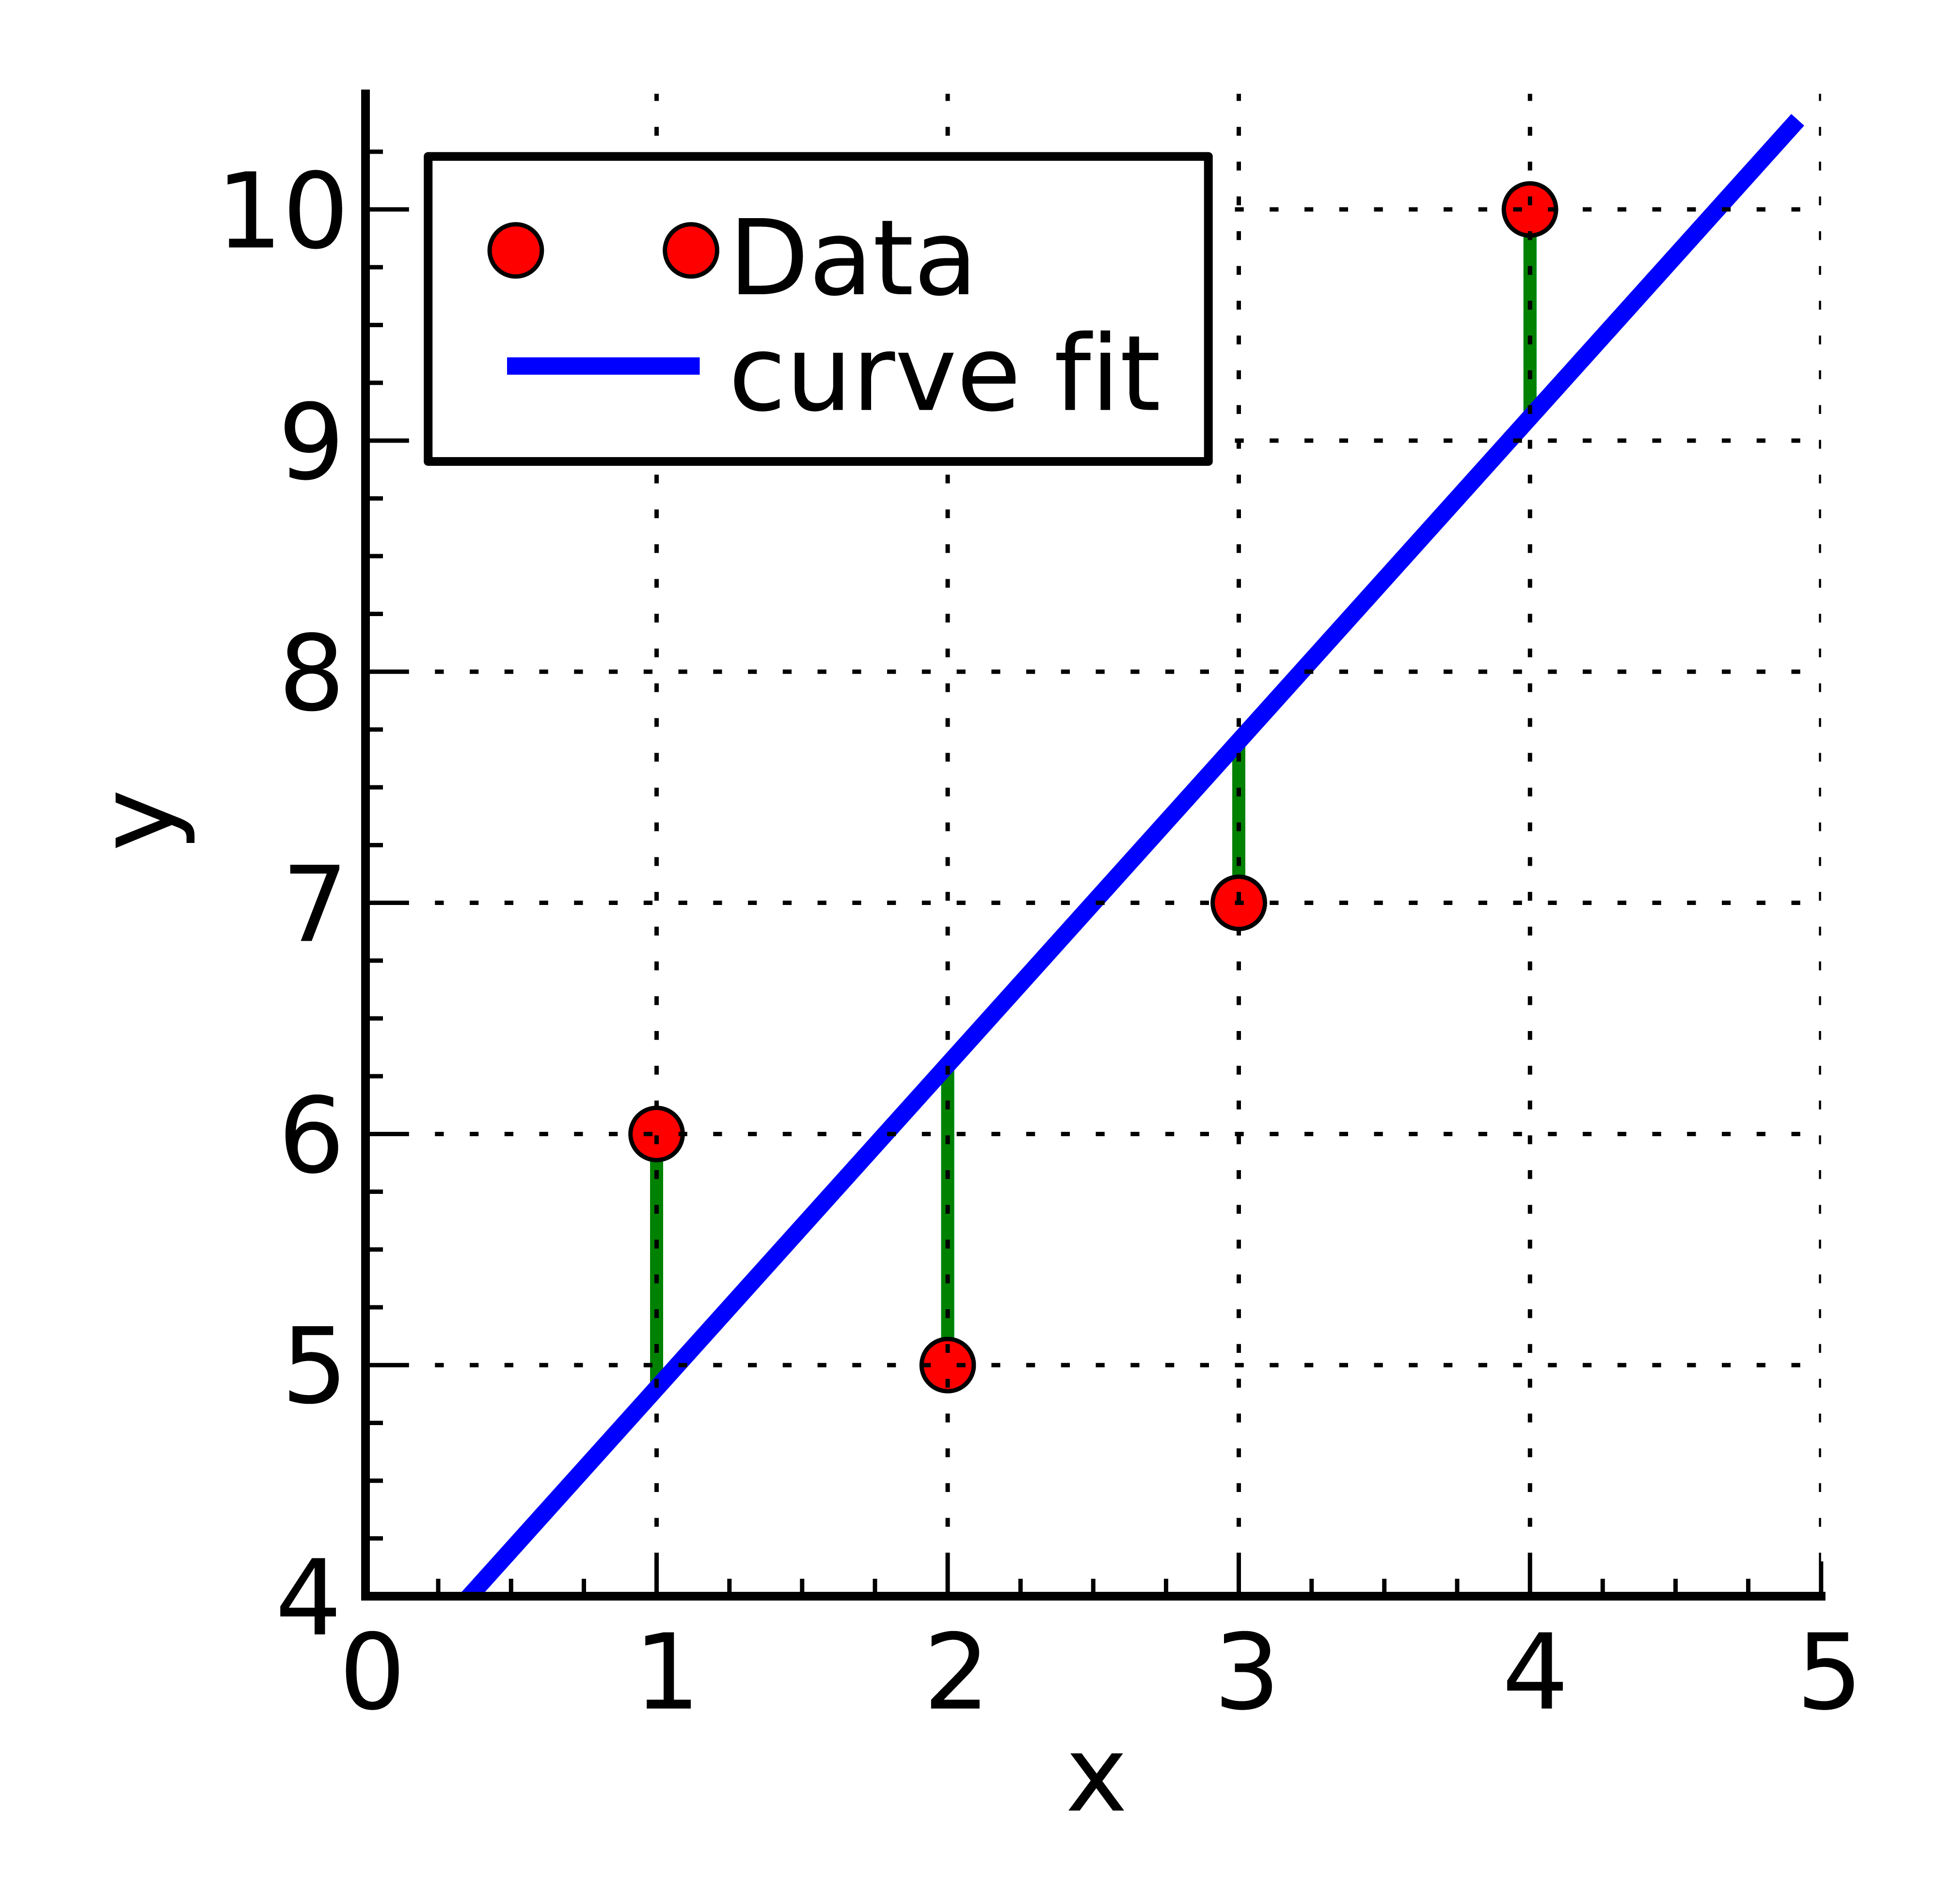
\includegraphics[width=0.5\linewidth]{src/Linear_regression.png}
    \footnote{\href{https://en.wikipedia.org/wiki/Linear_regression}{Wikipedia - Linear regression}}
  \end{center}
  % Añadir ejemplo estadística
\end{frame}

\begin{frame}{Ejemplos de funciones de perdida}
Principalmente se agrupan en:
\begin{itemize}
  \item \structure{\bf Perdida de regresión:} Dado un valor de entrada, el modelo predice el valor de salida. 
  
  \vspace{0.5em}

  Ejemplos: \textbf{Mean Squared Error, Mean Absolute Error...}

  $$MSE=\frac{1}{n}\sum_{i=1}^{n}(y^{(i)} - y_{pred}^{(i)})^2 $$
  $$MAE=\frac{1}{n}\sum_{i=1}^{n}| y^{(i)} - y_{pred}^{(i)}| $$
  \item \structure{\bf Perdida de clasificación:} Dado un valor de entrada, el modelo devuelve un vector de probabilidades de que la entrada pertencezca a una serie de categorias preestablecidas.

  \vspace{0.5em}

  Ejemplos: \textbf{Binary Cross Entropy, Categorical Cross Entropy...}

\end{itemize}
\end{frame}

\begin{frame}{Optimizadores}
Son algoritmos que se usan para \structure{\bf minimizar la función de perdida} o maximizar la función de ganancia.
Ejemplos: \alert{Adam, RMSprop, SGD...}
\vspace*{0.8em}

Cada vez que predecimos un valor mediante la red y comparamos con el valor real, \textbf{el optimizador ajusta los pesos de la red para minimizar la perdida.}
\begin{center}
  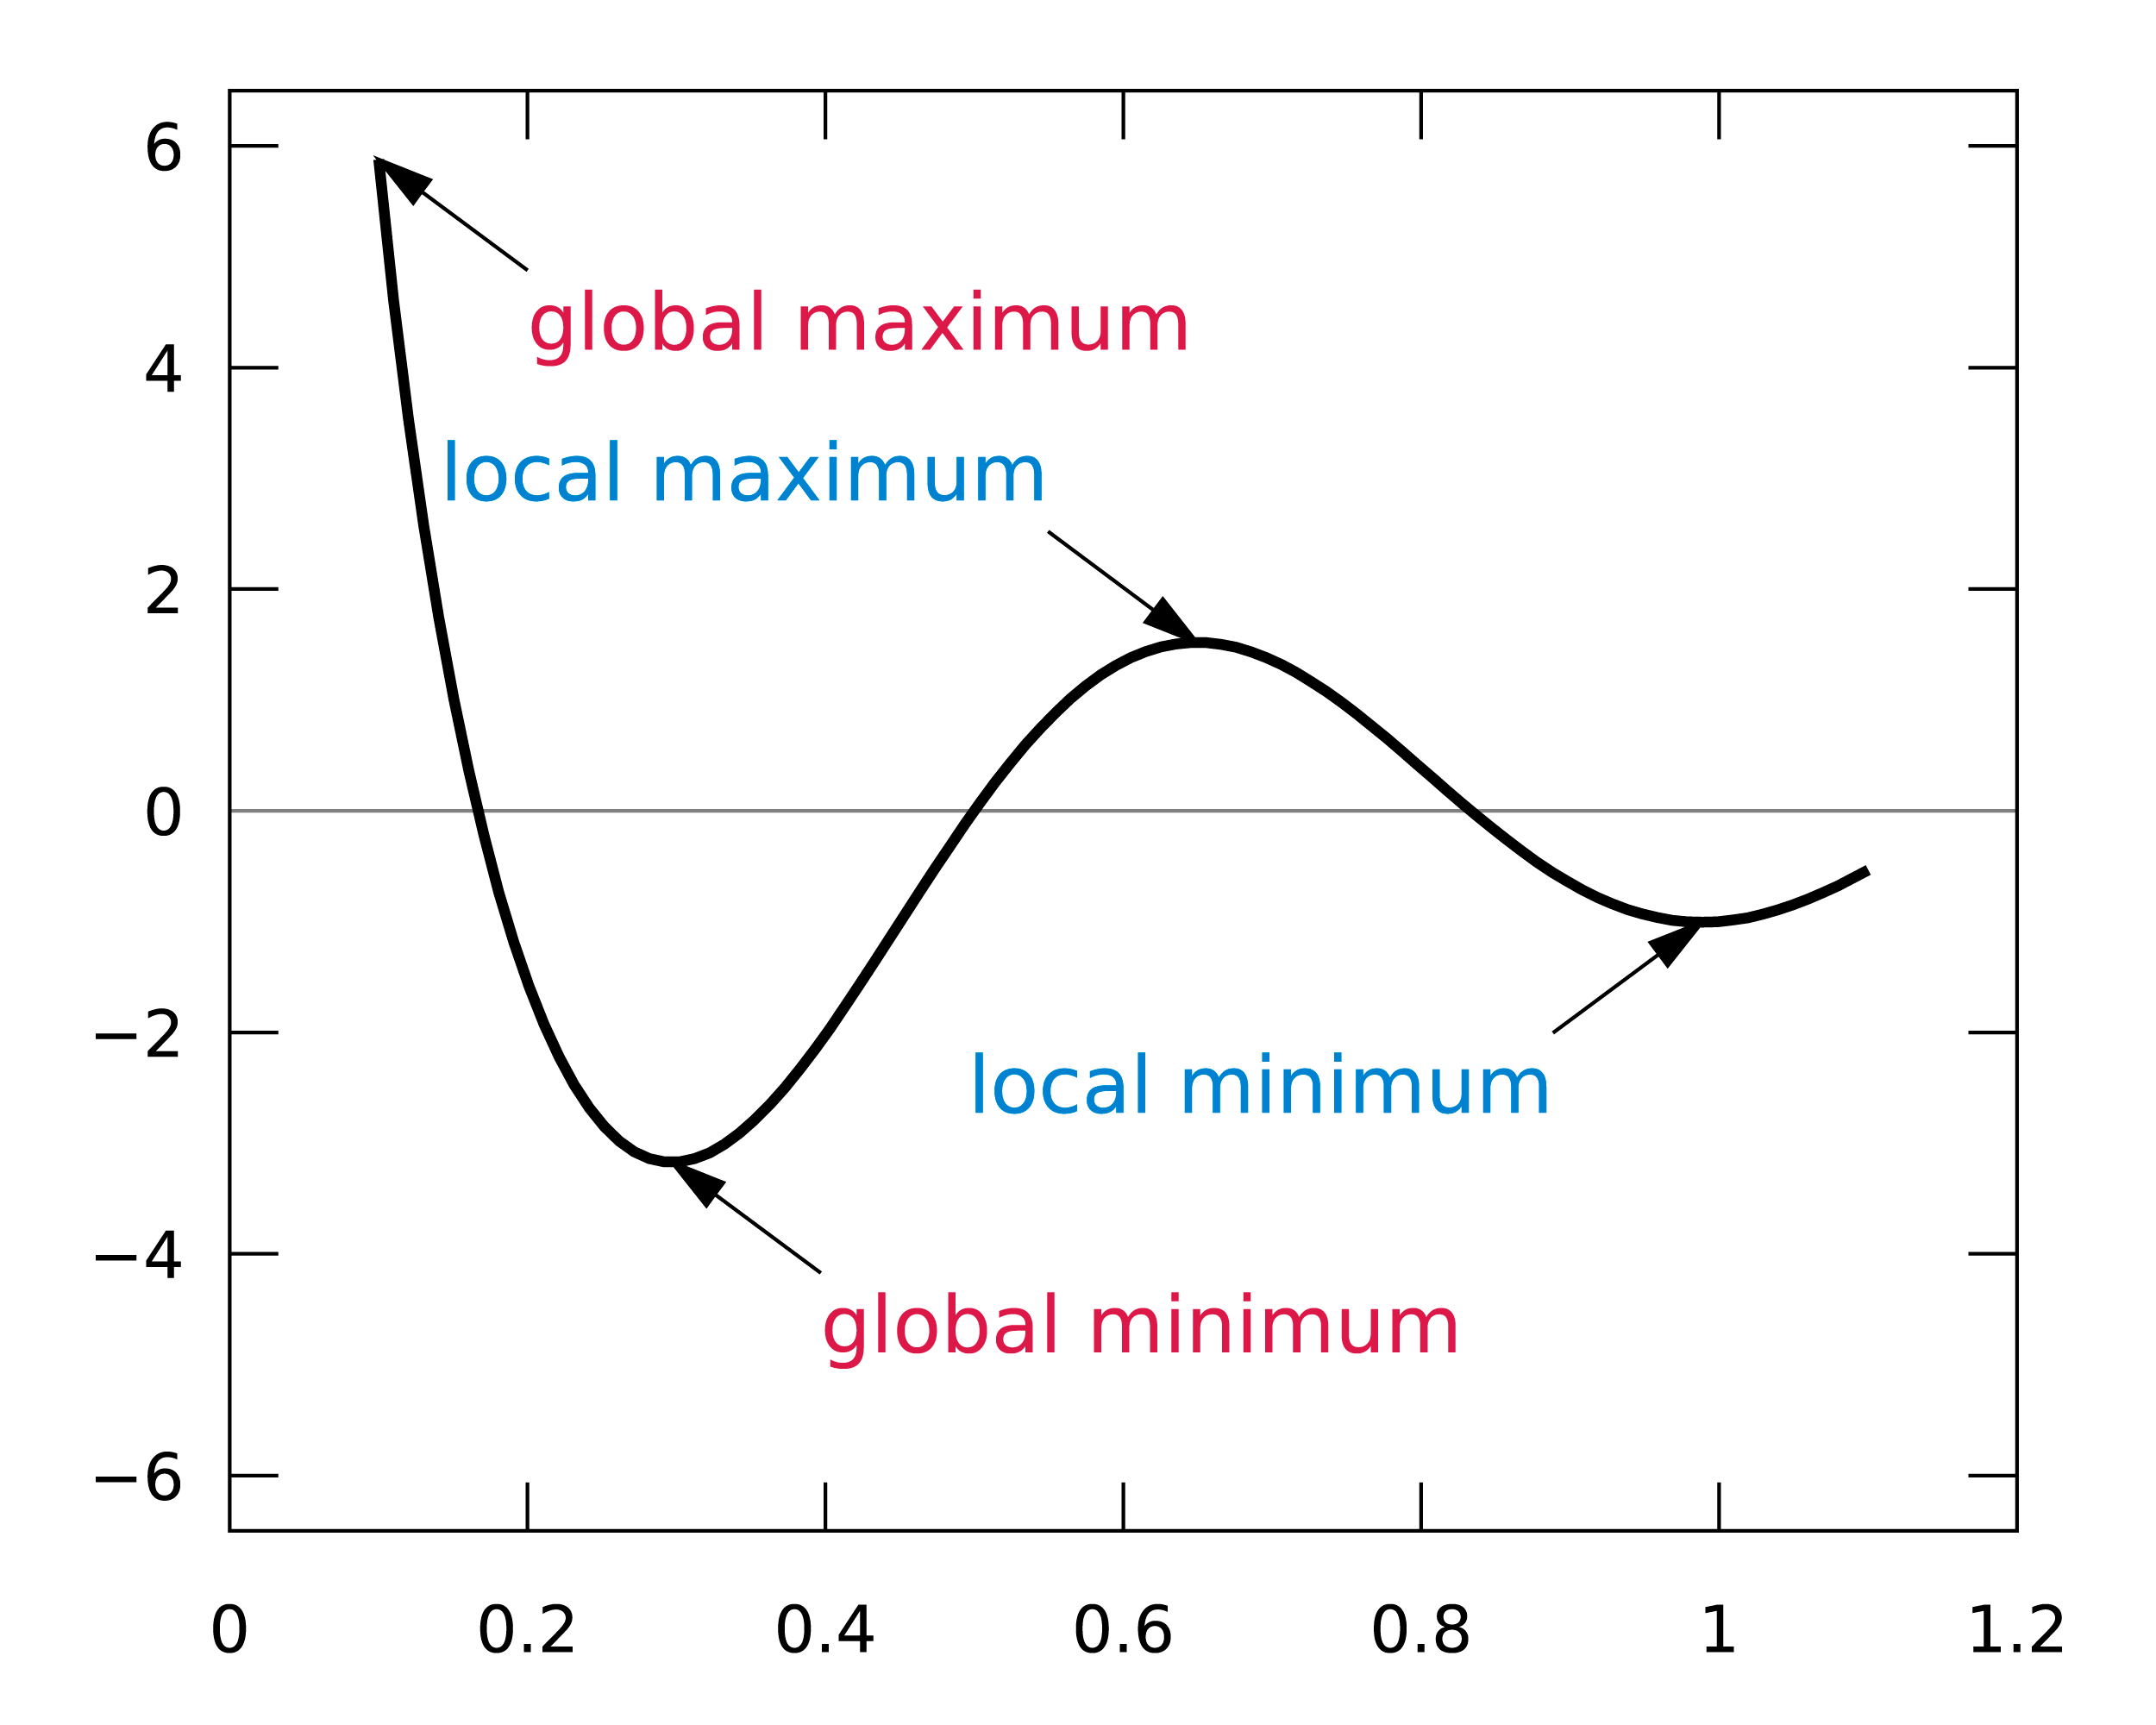
\includegraphics[width=0.5\linewidth]{src/Extrema_example_original.png}
\end{center}


Queremos obtener un mínimo global en la función de perdida. 

\end{frame}

\begin{frame}{Gradient Descent}
El algoritmo de descenso de gradiente es un \structure{\bf algoritmo de optimización que se utiliza para minimizar una función objetivo.}


Para implementarlo:
$$a_n+1=a_n - \delta \lambda F(a_n)$$

La idea es que el gradiente muestra la dirección de descenso entonces al movernos en esa dirección vamos a llegar a un mínimo, el problema es que puede ser un mínimo o un máximo.
% Añadir ejemplo imagen
% Añadir ejemplo web
\end{frame}

\begin{frame}{¿Cómo se calculan las derivadas?}
En ausencia de funciones de activación, la red neural es una función lineal, por lo que el gradiente de la función de perdida con respecto a los pesos de la red es una matriz de valores constantes.

En presencia de funciones de activación, la expresión como composición de funciones no es tan sencilla y se utilizan técnicas numericos llamadas Backpropagation.
\end{frame}

\begin{frame}{Hiperparámetros}
  Un hiperparámetro es un valor constante que se establece previo al  entrenamiento.
  Ejemplos: Tasa de aprendizaje, número de capas, número de neuronas, funciones de activación, funciones de perdida, optimizadores...

  Si un modelo no se comporta bien, entonces tenemos que modificar los hiperparámetros, ya sea para conseguir que el modulo aprenda más lento (tasa de aprendizaje), hacerlo más complejo (añadir más capas)\dots
\end{frame}
\begin{frame}{Tasa de aprendizaje}
  La tasa de aprendizaje define el tamaño de los pasos correctivas para que el modelo ajuste los errores en cada observación. Una tasa de aprendizaje muy alta
  provoca que el tiempo de entrenamiento sea menor, pero puede que el modelo no sea tan precioso. Por otro lado, una tasa de aprendizaje menor provoca un tiempo mayor de procesamiento, pero tiene el potencial de tener más precisión.

  % NO ES UNA CIENCIA EXACTA
\end{frame}

\begin{frame}{Batch Size}
  El tamaño del lote es el número de ejemplos de entrenamiento que se proporcionan a la red antes de que el optimizador actualice los pesos.

  Un buen tamaño de lote es generalmente 32. Pueden probarse: 32, 64, 128, 256...
\end{frame}

\begin{frame}{Numeros de epochs}
  Es el número de veces que se entrena la red con el conjunto de datos de entrenamiento.

\end {frame}

%% Añadir algo

\begin{frame}
  Principalmente hay dos frameworks que se utilizan:
  TensorFlow es una biblioteca de código abierto para aprendizaje automático a través de un rango de tareas, y desarrollado por Google para satisfacer sus necesidades de sistemas capaces de construir y entrenar redes neuronales para detectar y descifrar patrones y correlaciones, análogos al aprendizaje y razonamiento usados por los humanos.
PyTorch12 es una biblioteca de aprendizaje automático3 de código abierto basada en la biblioteca de Torch, utilizado para aplicaciones como visión artificial y procesamiento de lenguajes naturales, principalmente desarrollado por el Laboratorio de Investigación de Inteligencia Artificial4 de Facebook (FAIR).

% Añadir imagenes de tensorflow y pytorch

\end{frame}

\section{Ejemplos prácticos}
\begin{frame}{title}
  La idea de esta sección es ir mostrando una serie de ejemplos prácticos,
  para que se vea como se implementa una red neuronal en la práctica.

  Para ello tenemos que responder:
  ¿Es una red neuronal adecuada para nuestro problema?
  ¿Cuál va a ser nuestros datos de entrenamiento?
  ¿Cuál es nuestra arquitectura?
  ¿Qué hiperparámetros escoger?

\end{frame}
% Añadir cuando no es buena idea una red neuronal
\begin{frame}{Conecta4 AI}
Datos de entrenamiento
Mediante el algoritmo Minimax, se genera una tabla de entrenamiento que recoge para una posición del tablero, la mejor jugada que se puede hacer.
% \begin{table}[ht]
  \centering
  \begin{tabular}{|c|c|c|c|}
  \hline
  Estado Tablero 1 & Actua 2 & Mejor acción 3 \\
  \hline
 4949 & Valor 2 & Valor 3 & Valor 4 \\
  \hline
  \end{tabular}
  \caption{Tabla de ejemplo}
% \end{table}

%\url{https://es.wikipedia.org/wiki/Minimax#/media/Archivo:Minimax.svg}

\end{frame}

\begin{frame}{arquitectura}
  %% Insertar imagen arquitectura
\end{frame}

\begin{frame}{Convolución}
% https://towardsdatascience.com/conv2d-to-finally-understand-what-happens-in-the-forward-pass-1bbaafb0b148
Son muy importantes cuando tenemos que procesar imágenes, puesto
que ayudan a simplificar la imagen, para luego pasarlo por una capa densa y obtener un buen resultado.
\end{frame}

\begin{frame}{Hiperparámetros}
  train_size = 90000
  val_size = 5000
  test_size = 5000
  
  
  BATCH_SIZE = 64
  EPOCHS = 512
  LR = 0.001
  % Puedes tener todo bien y porque calcules mas la perdida da el ejemplo con un vector de clasificación
  %Añadir dos diferentes para completar y preguntar que creen que deberia de ser la perdida
    %LOSS = 'sparse_categorical_crossentropy'
\end{frame}

\begin{frame}{Criptografia AI}
Datos de entrenamiento
Imagenes aleatorias de tamaño 256x256
Texto aleatorio en formato ASCII


% Separar en 2?
Arquitectura: Autoencoder %iso Identidad
Encoder: Inccrusta el texto en la imagen devolviendo una imagen modificada.
Decoder: Devuelve el texto incrustado en la imagen.

\begin{center}
  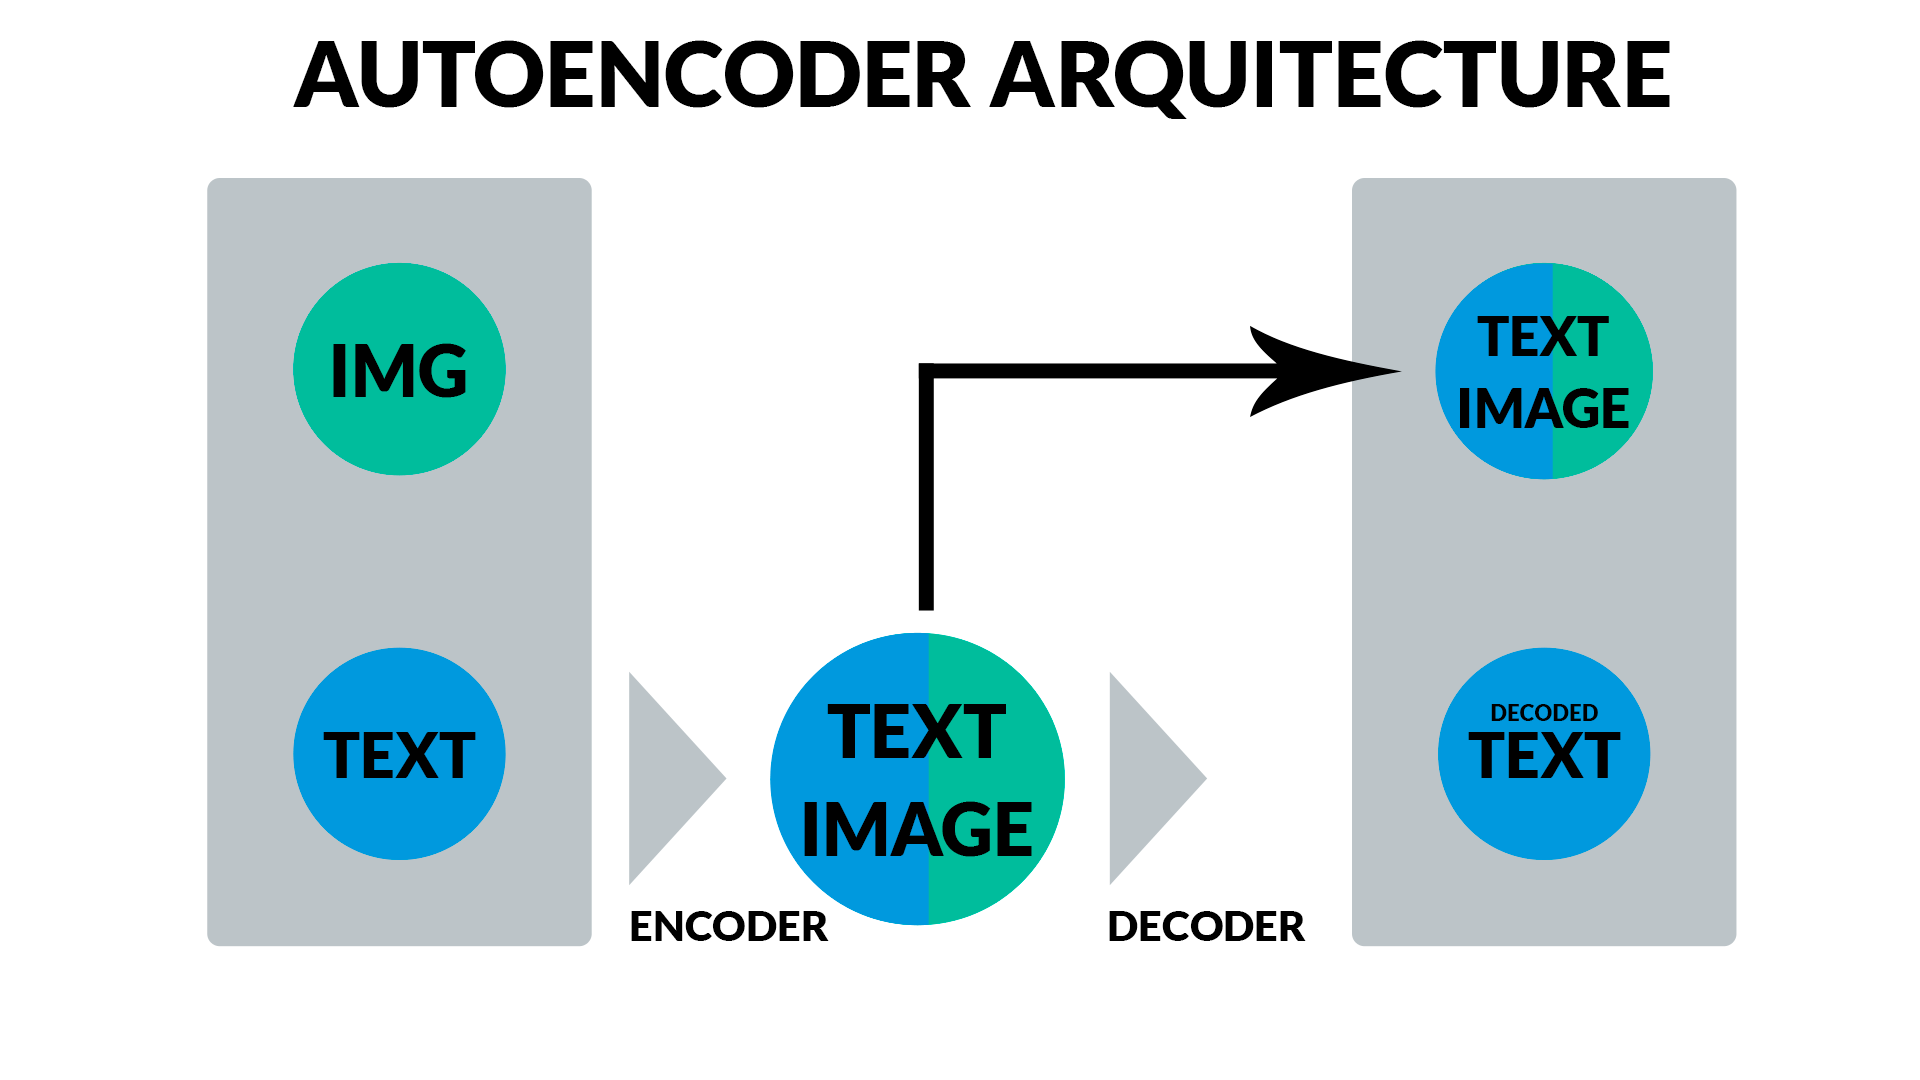
\includegraphics[width=0.5\linewidth]{src/AutoEncoder-arq.png}
\end{center}

\end{frame}

\begin{frame}{Encoder y Decoder}
  % Añadir imagen de encoder y decoder
  \begin{center}
    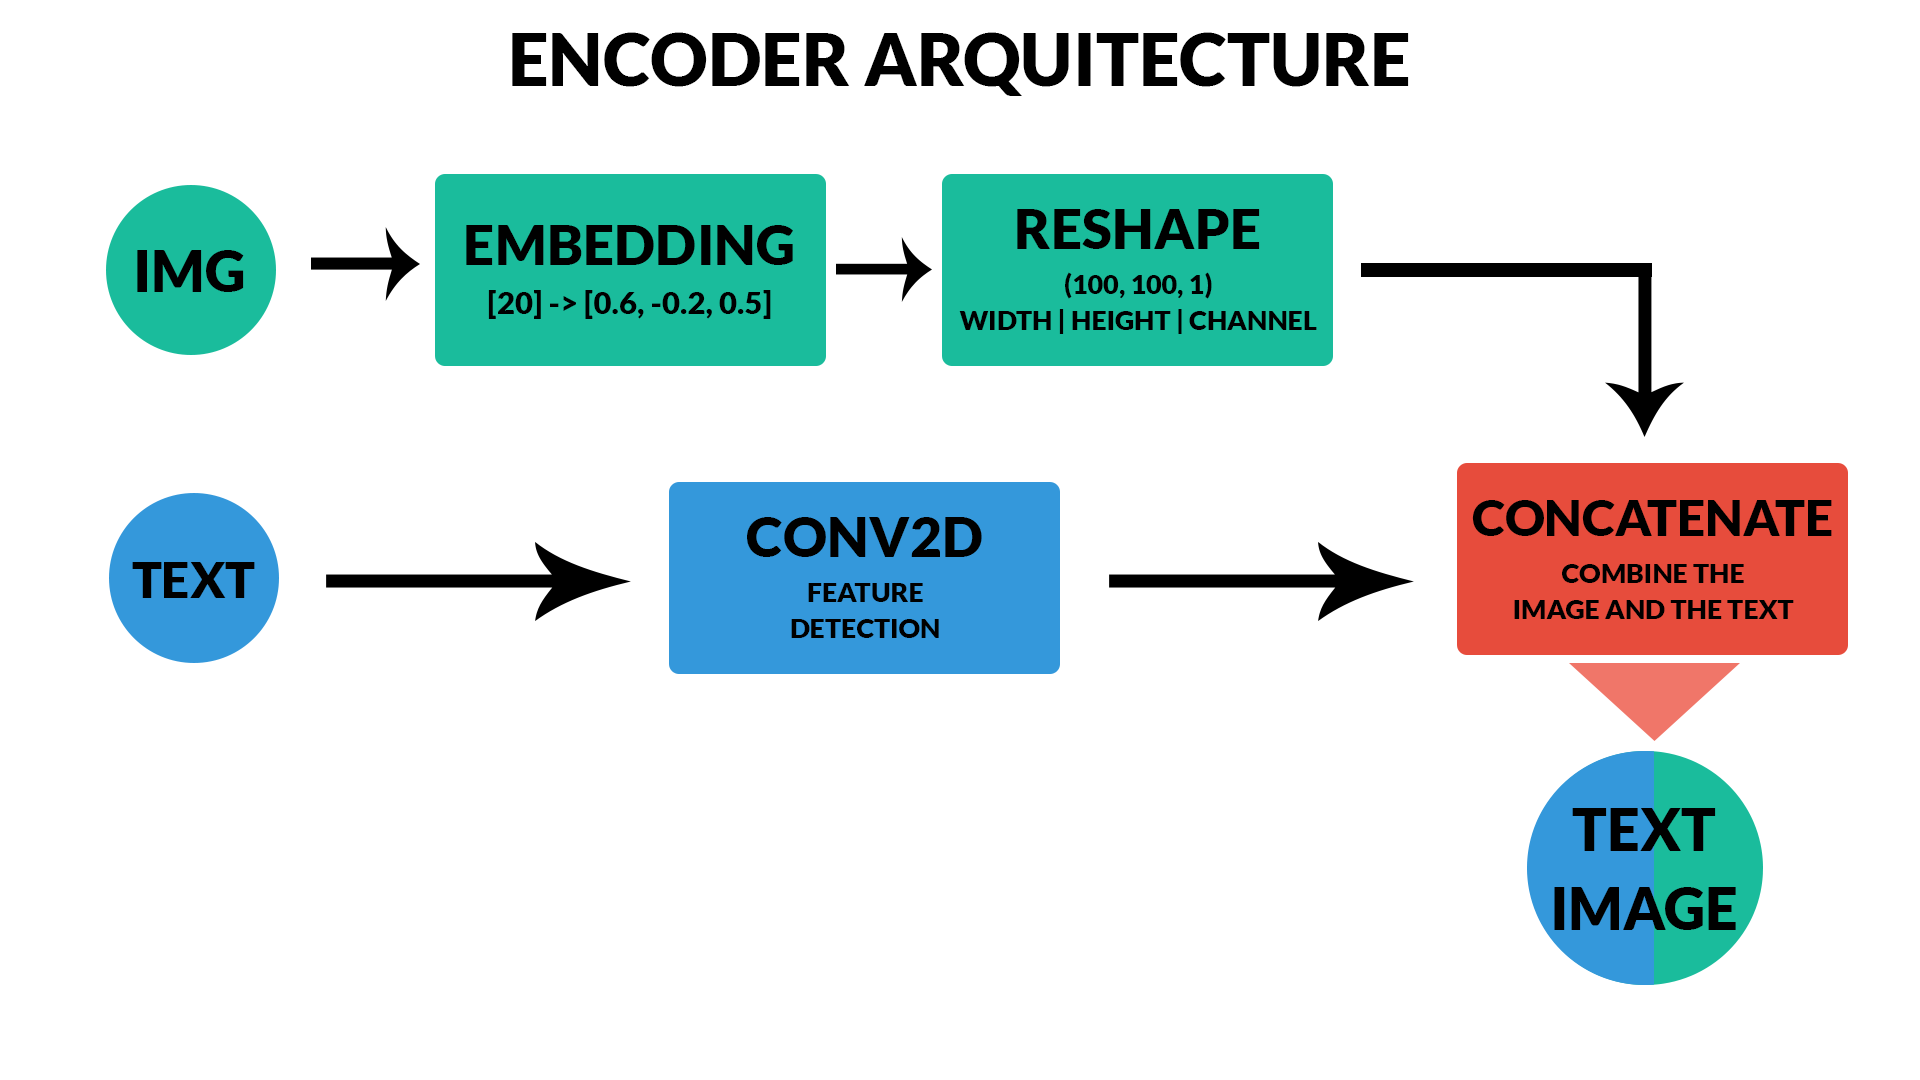
\includegraphics[width=0.5\linewidth]{src/Encoder-arq.png}
  \end{center}
  \begin{center}
    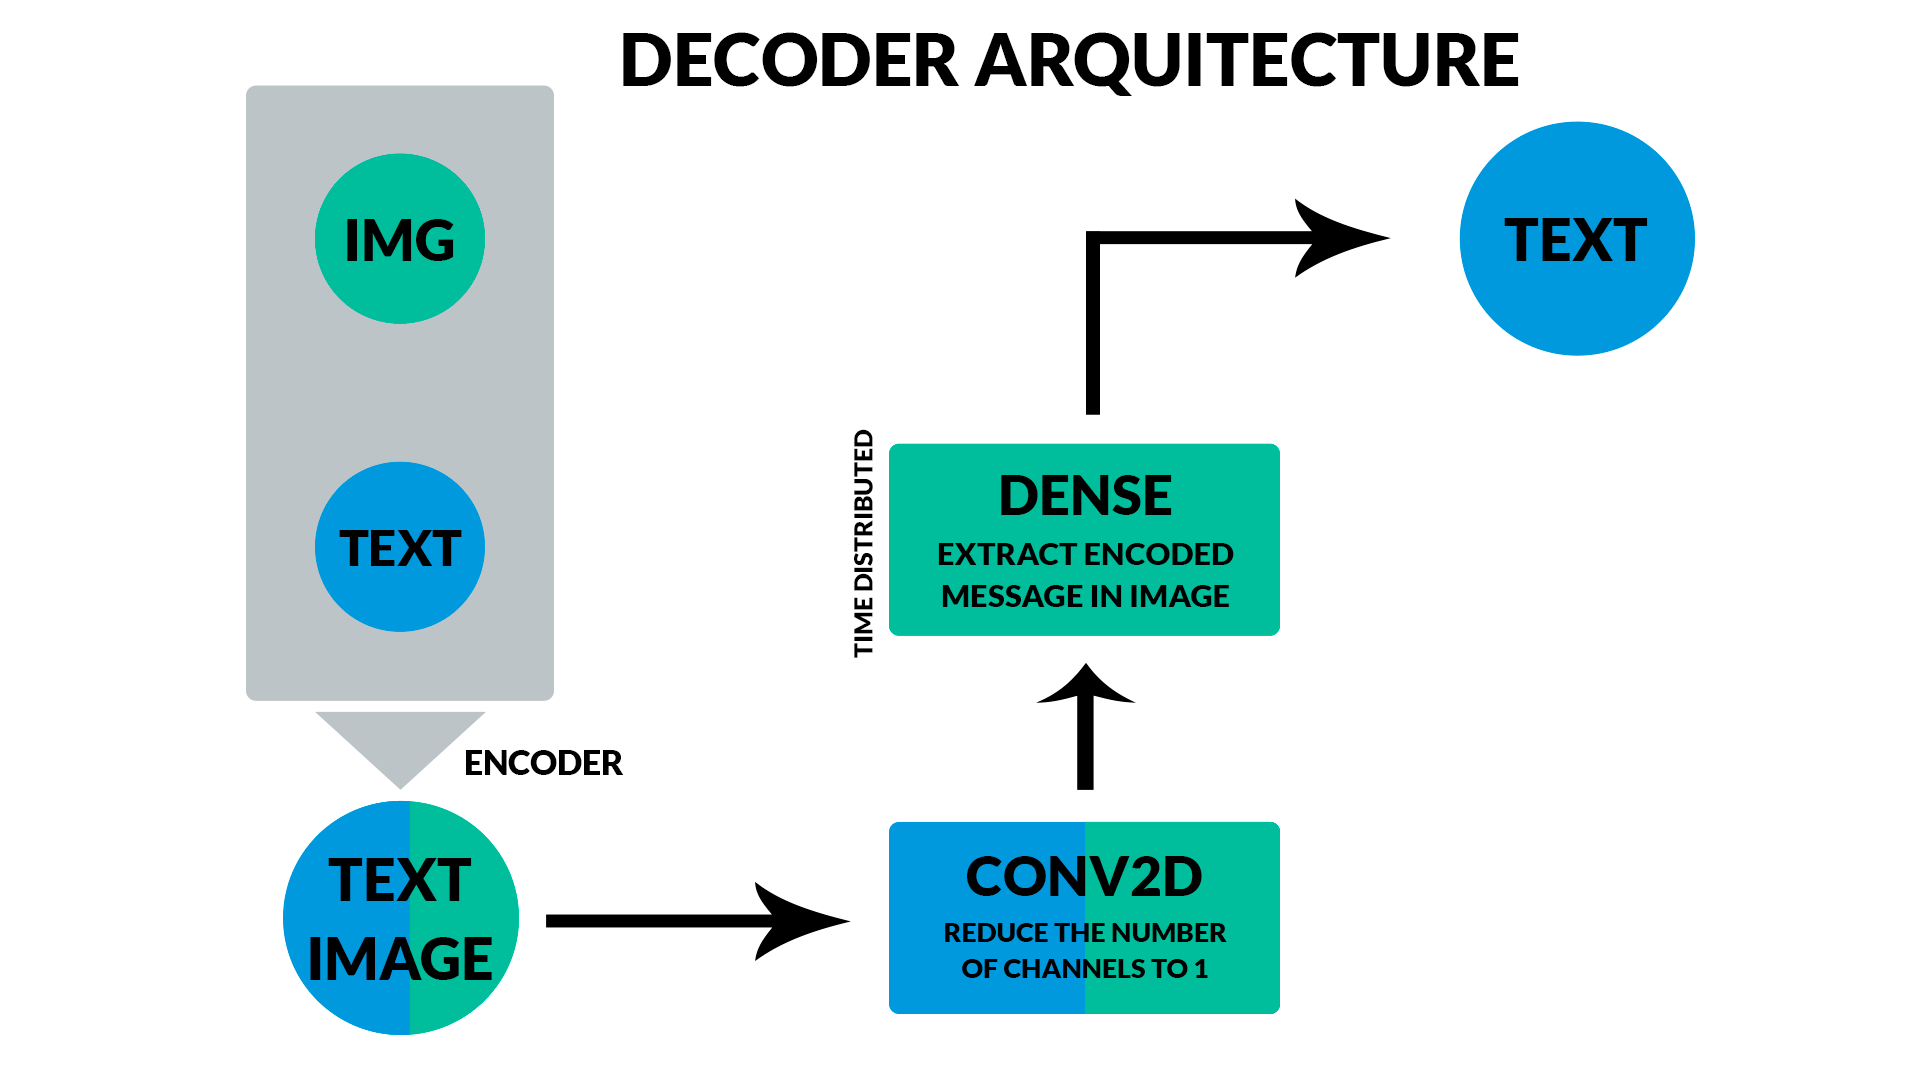
\includegraphics[width=0.5\linewidth]{src/Decoder-arq.png}
  \end{center}
\end{frame}

\begin{frame}{Hiperparámetros}
  % Añadir quizas la estructura en tf
  epochs=512, 
  steps_per_epoch=512,
  BATCH_SIZE = 64
  LR = 0.001

  Funciones de perdida?
  1º MSE
  2º Categorical Cross Entropy
\end{frame}

\begin{frame}{Doodle}
Base de Datos
% Añadir ejemplos de dibujos
\end{frame}

\begin{frame}{Arquitectura}
  % Añadir imagen de arquitectura
\end{frame}

\begin{frame}{Hiperparámetros}
  % Añadir quizas la estructura en tf
  epochs=512, 
  steps_per_epoch=512,
  BATCH_SIZE = 64
  LR = 0.001

  Funciones de perdida?
  1º MSE
  2º Categorical Cross Entropy
\end{frame}

\begin{frame}{ED}

\end{frame}



%--------------------------------------------------------------
\section{Ajuste de los parámetros}
%--------------------------------------------------------------

\begin{frame}{Aprendizaje supervisado}
%-------------------------------------
\begin{itemize}
  \item En redes supervisadas, se dispone de \structure{datos de entrenamiento}, formados por un conjunto de valores de entrada $\widehat x$, junto con los resultados asociados, $\widehat y$   
  \item Es usual disponer además de \structure{datos de test}, \texttt{xtest}, \texttt{ytest}
\end{itemize}
\end{frame}

\begin{frame}{Función de coste y entrenamiento de la red neuronal}
%-------------------------------------
\begin{itemize}
  \item El proceso de \alert{entrenamiento de la red neuronal} consiste en determinar los parámetros (pesos, $w_{j,k}^{(i)}$ y desplazamientos, $b_j^{(i)}$) que minimizan un funcional, "\alert{función de coste}", sobre los datos de entrenamiento:
  $$
  \Theta^* = 
  \mbox{argmin}\{ 
  J(\Theta; \widehat x, \widehat y), \quad \Theta=\left(w_{j,k}^{(i)}, b_j^{(i)}\right)\}
  $$
\item La función de coste varía con cada tipo de red neuronal. Por ejemplo, en problemas de regresión se suelen usar mínimos cuadrados ("\structure{MSE}: minimum mean square error"):
    $$
  J(\Theta; \widehat x, \widehat y) =
  \frac1{N_{data}} \sum_{i=1}^{N_{data}}
  \left(\widehat y_i - f_{NN}(\widehat x_i)\right)^2
  $$
\end{itemize}
\end{frame}

\begin{frame}{Algoritmos de minimización}

  \begin{itemize}
    \item Dificultades para la minimización: complejidad del funcional de coste, grandes valores de $N_{data}$
    \item Enormes requerimientos de cálculo para el entrenamiento, uso de grandes ordenadores, GPUs
    \item Se suelen utilizar algoritmos de tipo \alert{descenso de gradiente}\footnote{\url{https://en.wikipedia.org/wiki/Gradient_descent}}
    \[
      \Theta_{k+1} =  \Theta_k - \lr \nabla_\Theta{J(\Theta_k;\widehat x, \widehat y)}, \quad \mbox{\lr: "Learning Rate"}
    \]
  \item Necesidad de derivar de forma eficiente: \alert{diferenciación automática}\footnote{\url{https://en.wikipedia.org/wiki/Automatic_differentiation}}
    \item Algoritmos de \alert{gradiente estocástico}\footnote{\url{https://en.wikipedia.org/wiki/Stochastic_gradient_descent}}: en cada paso, se calcula el gradiente pero sólo en un subconjunto aleatorio de datos
  \end{itemize}
\end{frame}

\end{document}


%%% Local Variables:
%%% coding: utf-8
%%% TeX-master: t
%%% mode: latex
%%% ispell-local-dictionary: "english"
%%% End:
